\documentclass[twocolumn,floatfix,aps,prd,superscriptaddress,nofootinbib]{revtex4-2}

% Engine guard: glyphtounicode and \pdfgentounicode are pdfTeX primitives.
% Under LuaLaTeX/XeLaTeX they are undefined, the run aborts in the preamble,
% and every \cite comes out as "??".  LuaTeX and XeTeX emit correct ToUnicode
% maps on their own, so the block is simply skipped there.
\usepackage{iftex}
\ifPDFTeX
  \usepackage[utf8]{inputenc}
  \usepackage[T1]{fontenc}
  \usepackage{lmodern}
  \input{glyphtounicode}
  \pdfgentounicode=1
\else
  \usepackage{fontspec}
  \setmainfont{Latin Modern Roman}
  \setsansfont{Latin Modern Sans}
  \setmonofont{Latin Modern Mono}
\fi
\usepackage{graphicx}
\usepackage{amssymb}
\usepackage{amsmath}
\usepackage{xcolor}
\usepackage{hyperref}
\usepackage{textcase}
% placeins WITHOUT [section]: a two-column float can never be set on the page
% it is declared on, so a per-section barrier strands any figure* whose own
% section runs less than a page -- the next section's barrier flushes it to a
% float page of its own (Fig. 2 did this, 2026-09-18).  The barrier the paper
% actually needs is one, before the bibliography: that is where the LIGO
% figure had drifted to.
\usepackage{placeins}
\usepackage[protrusion=true,expansion=false]{microtype}

% A two-column strip plus its caption is about half a page, which the stock
% dbl-float parameters answer by giving it a page of its own and leaving the
% other half white (Fig. 2 did exactly that, 2026-09-18).  Raising the top
% fraction lets a wide float own most of a page's top, and raising the float
% -page fraction forbids a float page that would be less than three quarters
% full -- so a half-page strip has to ride at the top of a text page.
% REVTeX sets its own float parameters as the document opens, so these have
% to be applied after that, not in the preamble proper.
\AtBeginDocument{%
  \renewcommand{\dbltopfraction}{0.85}%
  \renewcommand{\dblfloatpagefraction}{0.75}%
  \renewcommand{\textfraction}{0.1}%
  \setcounter{dbltopnumber}{2}%
}

\graphicspath{{figures/}{../../../results/merger/figures/}}

\hypersetup{
    colorlinks=true,
    linkcolor=blue,
    filecolor=magenta,
    urlcolor=blue,
    citecolor=blue,
}
\urlstyle{same}
\emergencystretch=2em

\begin{document}

\title{\texorpdfstring{\MakeTextUppercase{From Spacetime Foam to Black-Hole Seeds: Merger and Scattering of Traversable Wormholes}}{From Spacetime Foam to Black-Hole Seeds: Merger and Scattering of Traversable Wormholes}}

\author{\MakeTextUppercase{Nikita M. Shirokov}}
\email{shirokov.nm@phystech.edu}
\affiliation{\textit{Independent Researcher, Moscow, Russia}}
\author{\MakeTextUppercase{Ilya Nachevsky}}
\email{ommnammashivaya@gmail.com}
\affiliation{\textit{Higher School of Economics, Moscow, Russia}}
\date{\today}


\begin{abstract}
We evolve pairs of massive Ellis--Bronnikov drainholes---traversable wormholes supported by a phantom scalar field---in 3+1 numerical relativity, at equal masses and one throat compactness, without spin. An isolated throat is an unstable fixed point: the sign of its perturbation selects collapse or inflation, with an e-fold time $\tau=5.9$ within $15\%$ of the Gonz\'alez--Guzm\'an--Sarbach rate. Like-signed scalar charges repel, so only opposite-signed pairs merge. The head-on merger forms a common horizon around both still-open throats---never one per throat---whose areal radius then shrinks by a quarter as it swallows the phantom field; the remnant rings down without a chirp. The spiral merger ends in a remnant of the same size: a shape-free finder recovers its common apparent horizon, $23\%$ deformed and invisible to star-shaped scans, five time units before a curvature wall that survives a $16\times$ refinement ladder and every gauge tried. No wormhole inspiral is possible: outliving even the vacuum inspiral time from the innermost stable circular orbit requires an initial perturbation below $10^{-20}$, so every encounter is a plunge. The most energetic gravitational-wave source is the horizonless fly-by, which radiates $(4$--$7)\times10^{-2}\,M$ in the dominant multipole---$16$--$29$ times the vacuum merger control and $40$--$70$ times a vacuum pass at its own momentum. The scalar field radiates comparable energy as a negative-energy $\ell=1$ dipole, which decays once a horizon forms. Rescaled to detector masses, the bursts match binary-black-hole templates at fixed duration (fitting factors $0.82$--$0.98$), but their frequency falls or drifts where a Kerr remnant's would hold; a $127$-template matched-filter search of $2.26$ h of Advanced LIGO O3b data finds no candidate. Collapse converts a throat of any astrophysical mass into a black hole of comparable mass within days. A primordial wormhole population would therefore supply halo-independent heavy seeds for the earliest supermassive black holes, evading the $\mu$-distortion bound on supermassive primordial black holes, together with a diffuse negative-energy scalar background and, for conversions at $z\approx20$, a sparse population of millihertz bursts whose time-averaged $\Omega_{\rm GW}\sim10^{-13}$--$10^{-11}$ at one seed per massive galaxy reaches LISA's sensitivity.
\end{abstract}

\maketitle

\section{Introduction}
\label{sec:intro}

Wheeler's spacetime foam is a sea of handles---wormholes that open and close on the Planck scale~\cite{wheeler1955,wheeler1957,misner_wheeler1957}. Several mechanisms promote them to macroscopic size: inflation stretches a Planck-scale Lorentzian wormhole with the background~\cite{roman1993}; bubble and domain-wall cosmologies produce post-inflationary regions joined through wormholes~\cite{garriga2016,deng2017}; and a gas of relic wormholes has been studied as a cosmology in its own right~\cite{kirillov2008,kirillov2011}. None of this work evolves the aftermath: what a macroscopic relic wormhole does, and what two of them do to each other. That is the subject of this paper.

Two classical facts govern the dynamics. First, the simplest evolvable traversable wormhole---the Ellis--Bronnikov drainhole held open by a ghost scalar~\cite{ellis1973,bronnikov1973,morris_thorne1988,visser1995}---is unstable: depending on the sign of the perturbation, the throat collapses to a black hole or inflates, on a timescale set by the throat radius~\cite{shinkai2002,gonzalez2009}, as 3+1 evolutions of the massless throat confirm nonlinearly~\cite{shirokov2026}. Second, Geroch's theorem forbids classical topology change~\cite{geroch1967,tipler1977}: two wormholes cannot fuse into one, and none can be created classically. Creation is quantum~\cite{hawking1988}, so our evolutions start at $t=0$ from the newborn state---the stipulated initial data of every numerical binary, here with a physical origin attached.

Together these facts set selection rules. No astrophysical assembly channel exists: a throat decays faster than dynamical friction or radiation reaction could pair it. A primordial pair born from foam needs no assembly---birth and collision coincide, at a separation comparable to the objects---and its evolution is a race between orbital collision and throat decay, both rates fixed by the classical solution. The scalar adds a second rule: a phantom field repels like charges and attracts opposite ones, so like-signed pairs scatter while opposite-signed pairs fall together; and the sign of a lone throat's perturbation selects collapse---a wormhole-to-primordial-black-hole channel beside the standard ones~\cite{zeldovich1967,carr_hawking1974,carr2021}---or inflation. A foam population thus splits into four fates---merger, scattering, collapse, inflation---across birth separation, perturbation and relative sign, the space mapped here. The binary evolved is the exterior approximation of a pair of handles (three asymptotic ends, the far sides passive), and what merges is not two wormholes into one, which Geroch's theorem forbids, but two wormholes into one black hole containing both throats.

The observable is not a chirp but a population of bursts from the merger epoch, redshifted into whatever band the mass scale selects~\cite{caprini2018,nanograv2023,lisa2017,lvk2021}. The epoch-independent deliverable is the energy radiated per event and its spectrum in throat-mass units, which converts any bound on $\Omega_{\rm GW}$---including the nucleosynthesis cap that holds outside every detector band~\cite{pagano2016}---into a bound on the abundance of primordial wormhole encounters. The collapse branch also bears on JWST's overmassive black holes at $z\gtrsim4$--$6$, which favour heavy seeds of $10^4$--$10^6\,M_\odot$ from formation channels that remain contested~\cite{bogdan2024,natarajan2024,greene2024,matthee2024,inayoshi2020}; Sec.~\ref{sec:discussion:seeds} develops it into a millihertz prediction.

Sections~\ref{sec:model} and~\ref{sec:setup} give the model and numerics. Sections~\ref{sec:single}--\ref{sec:spiral} follow the campaign from one throat to two: the lone wormhole, two throats at rest, and the head-on and spiral mergers. Section~\ref{sec:gw} treats the radiation of every channel, Sec.~\ref{sec:controls} the numerical controls, and Sec.~\ref{sec:ligo} confronts the rescaled waveforms with LIGO--Virgo--KAGRA data. Section~\ref{sec:discussion} draws the consequences and collects the open issues; Sec.~\ref{sec:repro} gives reproducibility and cost. All evolutions use \texttt{GRTeclyn}~\cite{grteclyn}, the AMReX-based~\cite{amrex} GPU port of \texttt{GRChombo}~\cite{grchombo}, continuing Refs.~\cite{shirokov2026,shirokov2026b}. We use $G=c=1$.

\section{The model}
\label{sec:model}

\subsection{Field equations}
\label{sec:model:field}

The matter is a single real, massless phantom scalar: gravity couples to \emph{minus} the canonical stress tensor,
\begin{equation}
T_{ab} = -\Bigl(\nabla_a\phi\,\nabla_b\phi - \tfrac12 g_{ab}\,\nabla_c\phi\nabla^c\phi\Bigr),
\qquad V(\phi)\equiv 0,
\label{eq:phantom}
\end{equation}
so $\rho<0$ where the gradient dominates---the exotic stress that holds a throat open. The field itself obeys the canonical wave equation $\Box\phi=0$, evolved in first-order form with $\Pi=(\partial_t\phi-\beta^i\partial_i\phi)/\alpha$.

\subsection{Drainhole initial data}
\label{sec:model:drainhole}

Each body is a massive Ellis--Bronnikov drainhole~\cite{ellis1973,bronnikov1973}. In isotropic radius $r$ about the throat centre, with
\begin{equation}
X = \frac{r - a^2/4r}{a},\quad
\Omega = 1 + \frac{a^2}{4r^2},\quad
u = \frac{m}{a}\Bigl(\arctan X - \frac{\pi}{2}\Bigr),
\end{equation}
the exact static solution of Eq.~\eqref{eq:phantom} is
\begin{equation}
\alpha = e^{u},\quad
\gamma_{ij} = e^{-2u}\,\Omega^2\,\delta_{ij},\quad
\phi = C\arctan X,
\label{eq:drainhole}
\end{equation}
with $4\pi a^2C^2 = a^2+m^2$, $K_{ij}=0$, $\Pi=0$ and zero shift; in the evolved conformal variables $\chi = e^{2u}\Omega^{-2}$ and $h_{ij}=\delta_{ij}$. Both constraints hold identically at $t=0$. Here $a$ is the throat scale and $m$ the ADM mass, carried by the lapse rather than the conformal factor, so $\chi$ at the throat stays in $[0.15,0.25]$ for $m/a\le1$ and mass costs no resolution. The minimal surface sits at $r_t=\tfrac12\bigl(m+\sqrt{m^2+a^2}\bigr)$ with areal radius $R_{\min}=e^{-u(r_t)}\sqrt{a^2+m^2}$; the production throat $a=2$, $m=1$ has $R_{\min}=3.8895$ at $r_t=1.618$. The point $r\to0$ is the far side's spatial infinity, compactified ($\chi\sim r^4$). At $m=0$ the throat is ultrastatic ($\alpha\equiv1$, $M_{\rm ADM}=0$) and two such throats do not attract.

\subsection{The binary superposition}
\label{sec:model:binary}

Two throats at separation $d$ (one-body radii $r_A$, $r_B$) are superposed in excess form,
\begin{equation}
u = u_A + u_B,\qquad
\psi = 1 + \bigl(\sqrt{\Omega_A}-1\bigr) + \bigl(\sqrt{\Omega_B}-1\bigr),
\end{equation}
with $\chi = e^{2u}\psi^{-4}$, $\alpha = e^{u}$ and $\phi = \phi_A + \sigma\,\phi_B$, $\sigma=\pm1$; the constant tail of the $\arctan$ profiles is subtracted so that $\phi\to0$ at the boundary. Momentum enters through one Bowen--York term~\cite{bowen_york1980} per throat,
\begin{equation}
\hat A_{ij} = \frac{3}{2r^2}\bigl[P_i n_j + P_j n_i - (\delta_{ij}-n_i n_j)\,P{\cdot}n\bigr],
\end{equation}
converted by $\tilde A_{ij} = \chi^{3/2}\hat A_{ij}$, with $K=0$. Since $\Pi=0$ the matter momentum density vanishes and $\hat A_{ij}$ is flat-space divergence free, so the momentum constraint holds \emph{exactly} at $t=0$; only the Hamiltonian constraint carries the superposition defect, $O(a^2/d^2)+O(m/d)$. The relative sign $\sigma$ is the pair's one discrete parameter. A phantom mediator \emph{repels} like scalar charges and \emph{attracts} opposite ones, with $Q\equiv|F_\phi/F_{\rm grav}| = (a^2+m^2)/m^2>1$ always ($Q=5$ for the production throat), so like-signed pairs never merge under their own gravity and $\sigma=-1$ is the merger channel. A windowed one-body correction of the Helfer type~\cite{helfer2022} is implemented but off in production (Sec.~\ref{sec:controls:systematics}).

\subsection{Declared seeds}
\label{sec:model:seeds}

The instability is probed with declared perturbations of the conformal factor only: a Gaussian shell on the minimal surface,
\begin{equation}
\psi \to \psi\bigl[1 + \varepsilon\, g(r)\bigr],\qquad
g = e^{-(r-r_t)^2/w^2},\quad w = a/4,
\label{eq:seed}
\end{equation}
which changes the throat's areal radius by a fraction ${\approx}2\varepsilon$, and a quadrupolar factor
\begin{equation}
\psi \to \psi\bigl[1 + \varepsilon_2\, g(r)\,P_2(\cos\theta)\bigr]
\end{equation}
about the $z$ axis through the throat. $K_{ij}$ and $\Pi$ are untouched, so the momentum constraint stays exact. The spherical seed selects the branch; the quadrupolar seed has no $\ell=0$ part and gives a collapsing throat a quadrupole to shed; with both on, the cross term is $O(\varepsilon\varepsilon_2)$.

\section{Numerical setup}
\label{sec:setup}

\begin{table*}[t]
\caption{The run matrix: $144$ evolutions in groups, each varying one knob against a named reference; per-run lines are in the shipped registry. Unless stated, $a=2$, $m=1$ ($R_{\min}=3.89$), $\sigma=-1$, $d=12$ and $L=64$. Left: the single throat, the pair, the head-on and the controls. Right: the orbital family.}
\label{tab:matrix}
\scriptsize
\begin{ruledtabular}
\begin{tabular}{llcc|llcc}
group & knob(s) & runs & Sec. & group & knob(s) & runs & Sec. \\
\hline
lone throat & levels 2--4; $\chi$ floor; $\Delta t$; $L{=}128$ & 9 & \ref{sec:single} & momentum scan & $p=0.20$--$0.45$ & 4 & \ref{sec:spiral:capture} \\
spherical kicks & $\varepsilon=\pm10^{-3}\ldots\pm10^{-1}$; level 4 & 9 & \ref{sec:single:branching} & fly-by, $p=0.45$ & level 5 on the doubled box & 2 & \ref{sec:gw:flyby} \\
quadrupolar kicks & $\varepsilon_2=0.005$--$0.05$; kick-free arm & 6 & \ref{sec:single:gw} & orbital chain, $p=0.12$ & $N$; levels; damping; $\chi$ floor & 13 & \ref{sec:spiral} \\
scalar-stream re-runs & unkicked level 4, $L{=}64$/$128$; $\varepsilon{=}{+}10^{-2}$ & 3 & \ref{sec:gw:censorship} & refinement ladder & levels 3--7; $\Delta t$; damping & 8 & \ref{sec:spiral:wall} \\
two throats at rest & $\sigma$; $a=1$--$3$; $d=12$--$18$; $p=0.12$ push & 9 & \ref{sec:pair} & interior freeze, $L{=}64$ & skin radii; arming time; extraction & 7 & \ref{sec:spiral:burst} \\
placement probes & $d=6$--$48$, one step each & 18 & \ref{sec:pair:placement} & wall probes & $p=0.15$--$0.25$; levels; fill off & 6 & \ref{sec:spiral:wall} \\
head-on, $d=8$ & fill; levels 3/5; down-step; $\pm\varepsilon$ & 10 & \ref{sec:headon} & production spiral, $L{=}128$ & three-stage chain; fill-window twin & 6 & \ref{sec:spiral:inspiral} \\
half-mass, $m=0.5$ & pair at $d=6$; lone control & 2 & \ref{sec:headon:halfmass} & Helfer twins & correction; window; levels & 6 & \ref{sec:controls:systematics} \\
vacuum BBH & same $d$, $p$, masses; no scalar & 3 & \ref{sec:controls:bbh} & gauge arms & $1{+}\log$ halved; harmonic; $\eta{=}4$; spiral, head-on & 10 & \ref{sec:spiral:wall} \\
constraint-solved data & \texttt{GRTresna} bridge & 1 & \ref{sec:controls:systematics} & shakedown (archived) & gauge, dissipation, tagging; boosted throat & 12 & \ref{sec:setup:scheme} \\
\end{tabular}
\end{ruledtabular}
\end{table*}

The campaign is one-knob: every run differs from a named reference in a single setting and has one line---difference, outcome, caveats---in the registry shipped with the results (Sec.~\ref{sec:repro}). Table~\ref{tab:matrix} groups the $144$ evolutions; $12$ form an archived shakedown that fixed the gauge, dissipation and tagging choices below and are not used for physics, leaving $132$.

\subsection{Evolution scheme}
\label{sec:setup:scheme}

We evolve CCZ4~\cite{alic2012} with damping $(\kappa_1,\kappa_2,\kappa_3)=(3,0,1)$, $1{+}\log$ slicing~\cite{bona1995} started from the exact static lapse of Eq.~\eqref{eq:drainhole}, a Gamma-driver shift~\cite{campanelli2006,baker2006} with $\eta=1$ started from zero, fourth-order stencils, RK4 and Kreiss--Oliger dissipation $\sigma=0.1$. The time step is $\Delta t=0.02\,\Delta x$, an order of magnitude below the usual CCZ4 Courant factor; the $\Delta t$ bracket that makes this necessary is a control (Sec.~\ref{sec:controls:systematics}).

\subsection{Grid, boundaries and regularisation}
\label{sec:setup:grid}

The domain is a cube of side $L=64$ centred on the system, with a $128^3$ base grid ($\Delta x=0.5$). Nested boxes, halving per level and centred on the tracked throats (half-width $4$ per throat at the production finest level), are re-drawn every $16$ steps. Production runs use three refinement levels (finest $\Delta x=1/16$); resolution arms go to levels $4$--$7$ where stated, and the orbital production chain and the fly-by use $L=128$, with the sponge and extraction spheres moved outward. Outer boundaries are Sommerfeld, backed by an absorbing sponge over $r=24$--$32$ whose extra dissipation ramps to $\sigma_{\rm sp}=4$ as the fourth power of the depth; everything dynamical stays inside $r=24$.

Each throat carries a compactified second infinity at its centre, where $\chi\sim r^4$, so the evolved variables are floored at $\chi\ge10^{-8}$ and $\alpha\ge10^{-10}$ (a variant floors $\chi$ at $10^{-20}$ and applies $10^{-8}$ only where $1/\chi$ is evaluated). Two further devices act only inside regions already trapped: exponential damping of the scalar where the lapse has collapsed, and an interior freeze that multiplies every right-hand side by $1-W(r)$, with $W$ a $C^2$ quintic step between radii $r_{\rm full}$ and $r_{\rm start}$. All three are numerical devices; twin runs measure whether any is load-bearing (Secs.~\ref{sec:headon:wall} and~\ref{sec:controls:systematics}).

\subsection{Diagnostics}
\label{sec:setup:diagnostics}

$L^2$ norms of the Hamiltonian and momentum constraints are written continuously. Both throat centres are tracked, and about each the areal radius $R(r)$ is scanned on coordinate spheres; its minimum is the throat. On the same spheres the null expansions $\theta_\pm$ are computed with the outward direction fixed by \emph{increasing areal radius}, so that a dynamic throat is marginally \emph{anti}-trapped~\cite{hochberg_visser1998}. The orientation matters: the in-code monitor fixes the outward direction by increasing \emph{coordinate} radius, which points the wrong way beyond a throat and manufactures trapped verdicts wherever $R(r)$ falls. Every horizon statement here is therefore read offline from archived plotfiles with the areal orientation; the in-code columns serve only as a live monitor.

The star-shaped scan reports the outermost coordinate sphere that is trapped everywhere ($\max\theta_+=0$, $\theta_-<0$). A trapped sphere lies inside the apparent horizon, so this sphere---``the scan's MOTS'' below---bounds the marginally outer trapped surface from inside. We quote its areal radius $R$ and its Misner--Sharp mass~\cite{misner_sharp1964},
\begin{equation}
\frac{2M_{\rm MS}}{R} \;=\; 1 + \frac{R^{2}\,\langle\theta_+\theta_-\rangle}{4},
\label{eq:misner_sharp}
\end{equation}
with the product averaged over the sphere. On an exact MOTS $M_{\rm MS}=R/2$; on the scan's spheres $M_{\rm MS}$ exceeds $R/2$ by up to ${\sim}13\%$ once a horizon has settled, and by up to $34\%$ while it forms. This is the shape systematic of star-shaped scanning, and it also affects whether a surface is found at all. Because the phantom violates the null energy condition, a trapped surface need not lie inside an event horizon; ``horizon'', ``censored'' and ``black hole'' below refer to MOTSs on the evolved slices. A deformable instrument backs the scan: a spectral flow finder expands the trial surface as $r=h(\theta,\phi)$ in real harmonics to $\ell=6$ ($8$ where stated) and drives its expansion to zero by a damped fast flow, with the same orientation rule. It recovers Kerr--Schild Schwarzschild ($R=2M$ to $0.03\%$ from spherical and dented seeds), correctly finds no surface on the time-symmetric Ellis throat ($\theta_-\ge0$ there), and reproduces the star-shaped scan on the head-on remnant to $2\%$.

Radiation is read from $\Psi_4$ on spheres at $R=10$, $14$, $18$ (and $22$ on the single-throat wave arms) for $L=64$ and at $R=20$, $28$, $36$, $44$ for $L=128$, decomposed in spin-weight $-2$ harmonics. Every amplitude quoted is $r\Psi_4$; the in-code and offline pipelines agree to $0.1\%$. The same spheres carry a scalar stream: $\phi$ and $\Pi$ in spin-weight-$0$ harmonics, $A_{\ell m}=R\,\phi_{\ell m}$, and the kinematic flux $F_{\rm kin}=-R^2\oint\Pi\,\partial_r\phi\,\mathrm{d}\Omega$, positive for an outgoing \emph{canonical} wave (Sec.~\ref{sec:gw:scalar}). A per-cell autopsy records the location and one-step history of any floating-point failure.

\section{The single wormhole}
\label{sec:single}

\begin{figure*}[t]
\centering
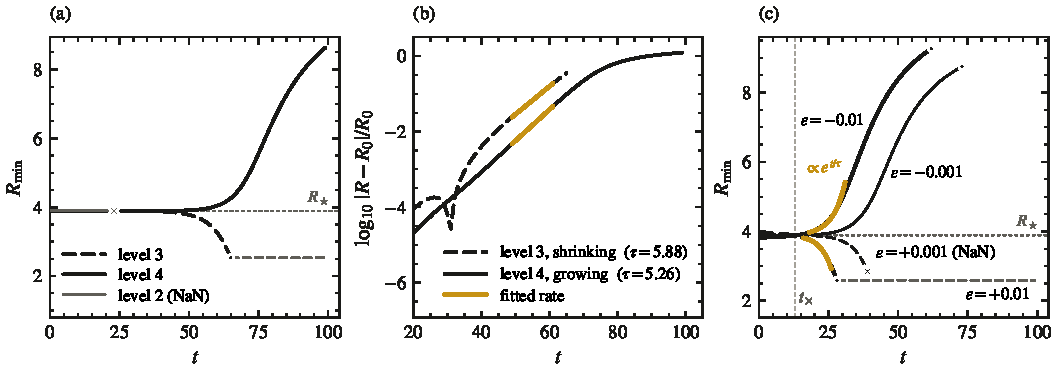
\includegraphics[width=0.80\textwidth]{01_single_throat/single_throat_instability.pdf}
\caption{Instability of the isolated throat. (a)~Minimal areal radius from exact static data at refinement levels 2--4. The exact solution ($R_\star$, dotted) is held until truncation noise excites the unstable mode: level 3 (dashed) collapses, level 4 (solid) inflates, level 2 (grey) dies of an origin failure first (cross). Dots mark where the scan loses the throat; muted lines carry the last reading. (b)~Deviation from $R_\star$: one exponential mode with a level-dependent sign, $\tau=5.88/5.26$ at levels 3/4. (c)~Level 3 with declared seeds, Eq.~\eqref{eq:seed}: $\varepsilon=\pm10^{-2}$ (heavy), $\pm10^{-3}$ (light); dashed, outward kicks. Twins cross at $t_\times\simeq13.0$ independent of $\varepsilon$. Gold: exponential fits; cross: the $+10^{-3}$ arm's death at $t=40.1$. (d),(e)~$L^2$ Hamiltonian and momentum norms (dash = sign, weight = amplitude, grey = no kick, crosses = deaths). A declared kick barely changes $\mathcal{H}$ at $t=0$ ($2.1$--$2.35\times10^{-3}$ for $|\varepsilon|\le10^{-2}$) and appears in $\mathcal{M}$ in proportion to $\varepsilon$ ($2.3\times10^{-4}$ at $10^{-2}$, $2.3\times10^{-5}$ at $10^{-3}$, against $2\times10^{-7}$ unkicked). All $|\varepsilon|\le10^{-2}$ arms then follow the unkicked norms, so the branching is not constraint-driven; only $\varepsilon=\pm0.1$ starts $3$--$6\times$ high, dying at $t=14.1$ ($+0.1$) and $15.2$ ($-0.1$) in a one-step overflow.}
\label{fig:single_throat}
\end{figure*}

\subsection{The static throat as a fixed point}
\label{sec:single:fixedpoint}

Evolved without a declared perturbation, the exact drainhole holds $R_\star=3.8895$ to $0.1\%$ for $35$ time units at level 3 and to $1\%$ until $t\simeq44$ (Fig.~\ref{fig:single_throat}(a)); at level 4 it is exact to four digits at $t=30$. The departure moves \emph{later} by $5.6$--$8.7$ units per halving of the cell---a truncation-noise seed of fixed growth rate handed a smaller amplitude. Level 2 dies of an origin failure at $t=24.2$ with the throat still exact to $0.12\%$. A lighter throat is less stable: at $m=0.5$ the throat holds $0.1\%$ only to $t\approx17$ and dies at its origin at $t=26.3$.

\subsection{The unstable mode}
\label{sec:single:instability}

The departure is a single exponential mode (Fig.~\ref{fig:single_throat}(a,b)): plateau fits give $\tau=5.88$ (level 3) and $5.26$ (level 4), i.e.\ $T\equiv\tau\,\alpha_{\rm th}/R_\star=0.87$ and $0.78$, where $\alpha_{\rm th}=e^{u(r_t)}=0.575$ is the static lapse at the throat, so that $T$ is the proper-time e-fold in units of the throat's light-crossing time. Gonz\'alez, Guzm\'an and Sarbach's perturbative growth times span $T=0.846$ at their massless end to $0.590$~\cite{gonzalez2009}; both measurements agree with that rate to ${\sim}15\%$ (a parameter-matched comparison has not been made). The seed is truncation error, and its sign flips with resolution---level 3 collapses, level 4 inflates---confirming from exact massive data the two branches found for the massless throat~\cite{shirokov2026}.

\subsection{Branching: collapse versus inflation}
\label{sec:single:branching}

A declared kick overrides the truncation seed (Fig.~\ref{fig:single_throat}(c)). At $\varepsilon=\pm10^{-2}$ and $\pm10^{-3}$ the fate is always opposite to the push, each $\pm$ pair crosses at the $\varepsilon$-independent $t_\times\simeq13.0$, and a tenfold smaller kick arrives $11$--$12$ units later at matched horizon radius---linear response on the same mode. The branching survives refinement: at level 4, whose own seed inflates the unkicked throat, $+10^{-2}$ still forms a horizon at $t=11$ and $-10^{-2}$ still inflates, the twins crossing at $t=12.99$ against level 3's $13.01$. The branch point is the throat's, not the grid's or the kick's. The kick also sets the clock: horizons form at $t=11$ ($\varepsilon=+10^{-2}$) and $t=25$ ($+10^{-3}$), against $t\le61$ for the unkicked throat (its first scanned slice after departure already holds a MOTS). At $\varepsilon=\pm0.1$ the data are no longer perturbative: both signs collapse and die ($t=14.1$ and $15.2$) from a Hamiltonian violation $3$--$6\times$ that of the $1\%$ arms (Fig.~\ref{fig:single_throat}(d,e)), so the usable range ends at $10^{-2}$.

\subsection{The collapse endpoint}
\label{sec:single:collapse}

The collapse branch ends in a black hole that consumes its supporting field. On the unkicked level-3 arm the horizon's areal radius falls $3.23\to2.37$ and $M_{\rm MS}$ $1.62\to1.23$ over $40$ units, with the origin lapse at $0.016$; the kicked $\varepsilon=+10^{-2}$ arm runs clean to $t=100$ behind its horizon. Unlike the massless throat of Ref.~\cite{shirokov2026}, which bounced at $t\approx4M$ and shed its horizon by $18.5M$, no arm here sheds a horizon. The pure-quadrupole arm ($\varepsilon_2=10^{-2}$, no radial kick) is fully instrumented (Fig.~\ref{fig:single_collapse}): a MOTS from $t=33$ at $R=3.80$, shrinking to $2.41$ ($M_{\rm MS}$ $1.90\to1.24$), while $|K|$ grows inward and the lapse pinches to zero at the centre.

The shrinking stops. In the three arms kicked with $\varepsilon=+10^{-2}$---at level 3, and at level 4 dressed with $\varepsilon_2=0.005$ and $0.05$---the horizon bottoms out near $t\approx47$, long before the pure-quadrupole arm reaches its floor, and grows back (Fig.~\ref{fig:single_regrowth}): by $9.7\%$ ($2.34\to2.57$), $8.8\%$ and $10.6\%$ in areal radius, with $M_{\rm MS}$ recovering $10$--$12\%$; the curves are smooth and saturating. The swallowed field's negative energy first shrinks the horizon and then, leaving, lets it regrow---the local counterpart of the negative-energy flux measured at infinity (Sec.~\ref{sec:gw:scalar}). Hawking's area law assumes the null energy condition~\cite{hawking1971}, which the phantom violates; this horizon runs it backwards, then forwards, in one evolution. The episode lasts minutes even at $10^{6}\,M_\odot$ (Table~\ref{tab:scales}); where the regrowth saturates is open at $t=100$.

\begin{figure*}[t]
\centering
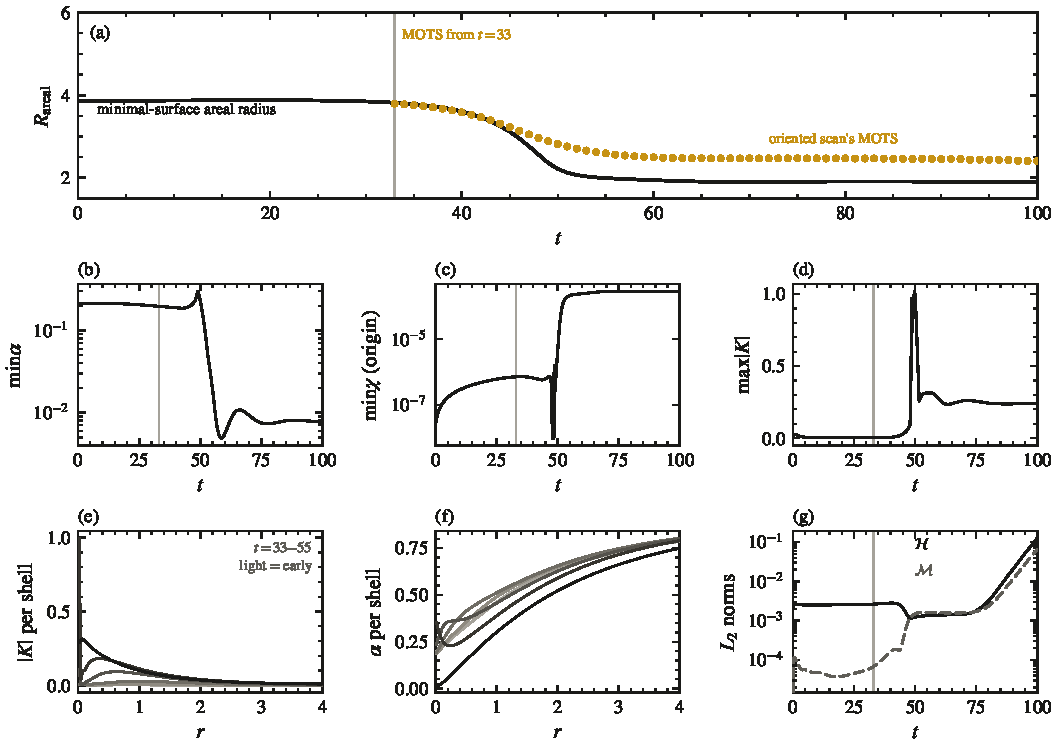
\includegraphics[width=0.80\textwidth]{01_single_throat/single_throat_collapse.pdf}
\caption{Collapse of the pure-quadrupole arm ($\varepsilon_2=0.01$, no radial kick). (a)~Minimal-surface areal radius (ink) and the scan's MOTS (gold) from $t=33$: $R$ $3.80\to2.41$, $M_{\rm MS}$ $1.90\to1.24$. Grey: the unkicked level-4 twin, which inflates on its own seed; this arm leaves it by $10\%$ only at $t=42$, against the kicked arm's $t=25$---the second-order drive of the pure quadrupole. (b)--(d)~Global $\min\alpha$, $\min\chi$ (the origin, the far side's compactified infinity) and $\max|K|$; the violent phase spans $t=45$--$55$. (e),(f)~Radial profiles over 128 shells, $t=33$--$55$ (light = early): $|K|$ grows inward while $\alpha$ pinches to zero at the centre. (g)~Constraint norms; the rise from $t\gtrsim75$ is the family's sphere-local floor growth, shared with the unkicked control.}
\label{fig:single_collapse}
\end{figure*}

\begin{figure*}[t]
\centering
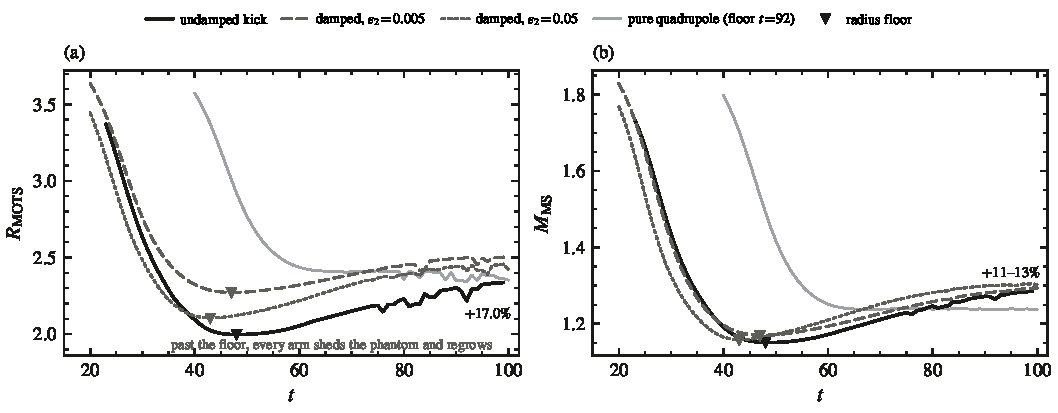
\includegraphics[width=0.80\textwidth]{01_single_throat/single_horizon_regrowth.pdf}
\caption{The remnant horizon shrinks and grows back: MOTS areal radius (a) and Misner--Sharp mass (b) of the three $\varepsilon=+10^{-2}$ collapse arms on the throat-centred scan, floors marked; the regrowth is $9$--$11\%$ in radius and $10$--$12\%$ in mass (Sec.~\ref{sec:single:collapse}).}
\label{fig:single_regrowth}
\end{figure*}

\begin{figure*}[t]
\centering
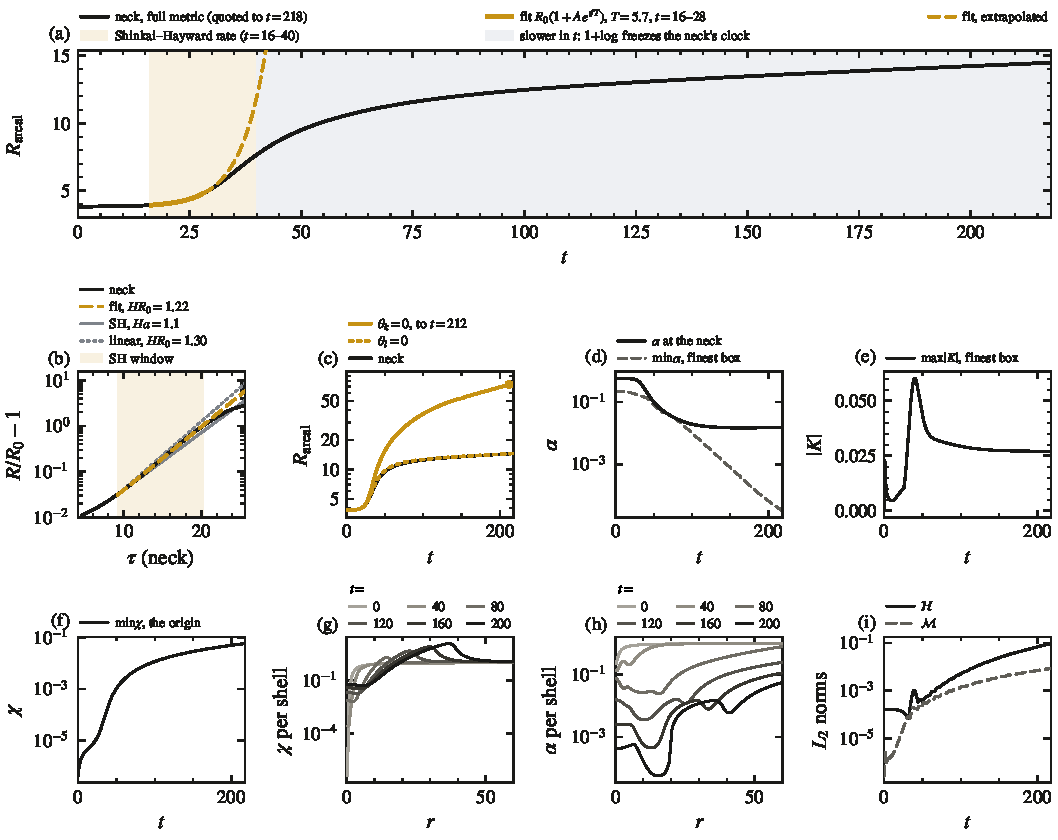
\includegraphics[width=0.80\textwidth]{01_single_throat/single_throat_inflation.pdf}
\caption{The inflation branch ($\varepsilon=-10^{-2}$, level 4), instrumented as Fig.~\ref{fig:single_collapse}. (a)~Minimal-surface areal radius (ink), $3.81\to11.39$ ($\times3.0$), against the unkicked level-4 twin (grey, $\times2.2$), the two parting by $10\%$ at $t=25$. Gold: scan rows carrying an anti-trapped shell ($\theta_\pm>0$), $t\approx1$--$36$. (b)--(d)~$\min\alpha$ falls $0.214\to0.080$, $\max|K|$ peaks at $0.057$ ($t=40.6$) and decays, and $\min\chi$ \emph{rises} $2.4\times10^{-8}\to1.4\times10^{-3}$---each opposite to the collapse branch. (e),(f)~Shell profiles to $r=4$ (light = early): the inner sheet's $\chi$ trough moves outward, to $r\approx1.4$ by $t=100$; spurious $\theta_+=0$ rows at $R\approx61$ after $t=85$, where the trough crosses a scan sphere, are not drawn. (g)~Constraint norms hold to $t\simeq50$ and grow $60\times$ in $\mathcal{H}$ by $t=100$; the record is quoted only where the mode is exponential.}
\label{fig:single_inflation}
\end{figure*}

\subsection{The inflation branch}
\label{sec:single:fate}

The inflation branch forms no horizon. The $\varepsilon=-10^{-2}$ arm at level 4, instrumented like the collapse arms (Fig.~\ref{fig:single_inflation}), grows $3.81\to11.39$ in areal radius by $t=100$ with no trapped surface anywhere, carrying instead anti-trapped shells ($\theta_\pm>0$) on the scans over $t\approx1$--$36$. It leaves its unkicked level-4 twin, which inflates on its own truncation seed, by $10\%$ at $t=25$---when the $+10^{-2}$ twin on the same level has already formed its horizon---and rides the same mode. The growth is not a runaway. While the deviation is small it grows at the mode's $0.190\pm0.002$ per unit, but once the radius has doubled $\mathrm{d}\ln R/\mathrm{d}t$ peaks and decays: from $0.031$ near $t\approx75$ to $0.010$ at $t=99$ in the unkicked arm (doubling time $22\to67$), and $0.036\to0.0023$ in the kicked one ($19\to298$). A box-doubled ($L=128$) copy of the unkicked arm tracks it to $0.3\%$ in $R$, so the boundary plays no role. The collapse runs away; the inflation coasts.

Its end state is open, and the throat is shedding its own support: the monopole scalar flux through every sphere grows quasi-exponentially over the quotable window (Sec.~\ref{sec:gw:censorship}). Three endings remain: saturation at a larger radius, disfavoured because static drainholes are unstable fixed points; unbounded coasting, as in the spherical literature~\cite{shinkai2002}; or a turnover into collapse once too little phantom support remains, which a flux still growing when its reservoir is spent would force. A downturn of $R_{\min}(t)$ followed by a trapped surface would decide it. None occurs by $t=100$, beyond which the constraint norms leave their floor ($t\gtrsim80$ in both boxes).

\subsection{Lifetime and physical scale}
\label{sec:single:lifetime}

At fixed $m/a$ the solution is scale-free, and the measured e-fold is $\tau\alpha_{\rm th}=0.78$--$0.87\,R_\star$ in proper time---one light-crossing of the throat. The lifetime is a logarithm of the seed: a horizon at $11\,M$ for $\varepsilon=10^{-2}$ and $25\,M$ for $10^{-3}$, a decade costing $14\,M\simeq\tau\ln10$; the unkicked throat's horizon by $61\,M$ places the level-3 truncation seed at $\varepsilon\gtrsim2\times10^{-6}$. Table~\ref{tab:scales} converts these to physical units. No static throat of astrophysical mass survives: a stellar-mass drainhole is gone in milliseconds, a supermassive one in minutes, and only at $10^9\,M_\odot$ does the lifetime reach days. The logarithm makes this robust: ten further decades of quiet initial data extend a $30\,M_\odot$ throat from $1.6$ to $22$ ms. A foam-born pair must collide as it is born or not at all (Sec.~\ref{sec:discussion:noinspiral}).

\begin{table}[t]
\caption{The drainhole clock in physical units: the production throat ($R_\star=3.89\,M$) scaled by its ADM mass $M$. $\tau=5.9\,M$ is the e-fold time (Sec.~\ref{sec:single:instability}); the last three columns are the measured times to a horizon for the two declared kicks and an upper bound for truncation noise (Sec.~\ref{sec:single:branching}). Intermediate seeds follow $t_{\rm BH}\simeq11\,M+\tau\ln(10^{-2}/\varepsilon)$.}
\label{tab:scales}
\scriptsize
\begin{ruledtabular}
\begin{tabular}{lccccc}
 & & & \multicolumn{3}{c}{time to a horizon} \\
$M$ & $R_\star$ & $\tau$ & $\varepsilon=10^{-2}$ & $10^{-3}$ & noise ($\le$) \\
\hline
$30\,M_\odot$ & $172$ km & $0.87$ ms & $1.6$ ms & $3.7$ ms & $9.0$ ms \\
$10^{3}\,M_\odot$ & $5.7\times10^{3}$ km & $29$ ms & $54$ ms & $0.12$ s & $0.30$ s \\
$10^{6}\,M_\odot$ & $5.7\times10^{6}$ km & $29$ s & $54$ s & $2.1$ min & $5.0$ min \\
$10^{9}\,M_\odot$ & $38$ AU & $8.1$ h & $15$ h & $1.4$ d & $3.5$ d \\
\end{tabular}
\end{ruledtabular}
\end{table}

\section{Two throats at rest}
\label{sec:pair}

\begin{figure*}[!t]
\centering
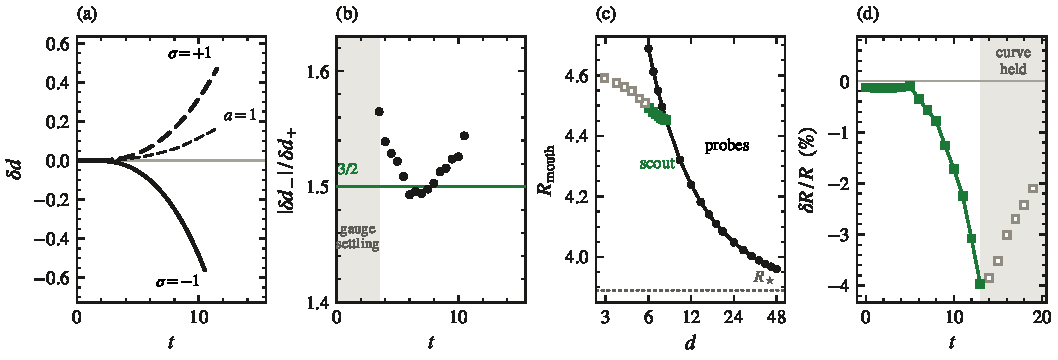
\includegraphics[width=0.80\textwidth]{03_two_throats/pair_interaction.pdf}
\caption{Two throats at rest: the sign rule (a,b) and its calibration (c,d). (a)~Separation change of three $d=12$ pairs one knob apart: like-signed ($\sigma=+1$, heavy dashed) opens, opposite-signed ($\sigma=-1$, solid) closes, and the narrow like-signed pair ($a=1$, light dashed) opens $2.8\times$ more slowly. Separations are inverse-$\chi$-weighted centroids of the midplane $\chi$ pits. (b)~Pull-to-push ratio against the prediction $(Q{+}1)/(Q{-}1)=3/2$ for $Q=5$ (gold): measured $1.518\pm0.021$ (scatter over $15$ slices); grey, the gauge-settling window $t<3.5$, excluded. (c)~Per-mouth areal radius of freshly placed pairs at $t=0$ (circles), exceeding the isolated $R_\star$ (dotted) by an excess $\propto d^{-1.16}$. Gold squares: the head-on scout's mouths at the separation reached; open grey squares (here and in d) lie closer than the closest probe. (d)~The scout against the placement curve, $\delta R/R=R_{\rm scout}/R_{\rm place}-1$: the $-0.13\%$ plateau to $t=5$ calibrates the tracker's grid snap, and the squeeze then grows to $-4.0\%$ by $t=13$. In the shaded band the curve is held at its last point, so the magnitude is a lower bound; a boost can only raise a coordinate-sphere reading, so a reading below the curve is a genuine squeeze.}
\label{fig:pair}
\end{figure*}

\subsection{The sign rule}
\label{sec:pair:sign}

Two identical throats released from rest push apart; reversing one throat's scalar turns the push into a pull (Fig.~\ref{fig:pair}(a,b)). Both forces share one radial law, so their ratio $Q$ is separation-independent: no gap, mass or approach speed lets a like-signed pair fall together, and $\sigma=-1$ is the only gravity-driven merger channel. The flip is not a tuning: $\phi\to-\phi$ leaves $T_{ab}$, and with it the one-body geometry, unchanged. The measured pull-to-push ratio at $a=2$ is $1.518\pm0.021$ (scatter over $15$ slices) against the predicted $(Q+1)/(Q-1)=3/2$, and the force follows the throat width---the scalar charge---not the mass, which is equal in all arms.

\subsection{The force law}
\label{sec:pair:force}

Four like-signed pairs, identical but for the gap, are displaced at a common $t=11.5$ by $0.4696/0.3699/0.2980/0.2438$ for $d=12/14/16/18$. Inverse-square in the coordinate separation is excluded---$F\,d^2$ rises monotonically $67.6\to79.0$ across the ladder---but $F\propto(d+\delta)^{-2}$ with $\delta\approx3$--$4$ describes it: $\delta$ fitted on $d=12$--$16$ alone predicts $0.246$ at $d=18$, where inverse-square gives $0.209$ and the measurement is $0.2438$. Since $\delta$ is comparable to the placed pair's mouth radius ($4.24$ at $d=12$; Sec.~\ref{sec:pair:placement}), the force is inverse-square in an \emph{effective} separation exceeding the coordinate one by about a throat radius. Across widths the push grows at every rung ($0.147/0.283/0.416/0.615$ for $a=1/1.5/2/3$) with an effective exponent of $1.3$--$1.4$; the point-charge $a^2$ scaling is not confirmed.

\subsection{Placement systematics}
\label{sec:pair:placement}

Freshly placed pairs read $+1.8\%$ ($d=48$) to $+20.5\%$ ($d=6$) wider than the isolated throat, falling as $d^{-1.16}$ (Fig.~\ref{fig:pair}(c,d)), so every same-$d$ comparison here is made against that curve rather than against the lone throat. Read that way, the released head-on pair's mouths are genuinely squeezed, $-0.6\%$ at $t=7$ growing to $-4.0\%$ by $t=13$---an interaction effect, since the lone throat holds its radius to $0.1\%$ until $t\approx35$.

\section{The head-on merger}
\label{sec:headon}

\subsection{Contact and the common horizon}
\label{sec:headon:contact}

Released from rest at $d=8$ with opposite scalar signs, the pair reaches contact at $t\approx20$ while both mouths are still open, and a common MOTS encloses them from $t=22$: the corrected scan finds it at $r=3.17$ with areal radius $R=5.56$ ($M_{\rm MS}=2.99$; Fig.~\ref{fig:headon_collapse}). No scan finds a surface about either mouth at any time: the horizon is born common. Its irreducible mass $R/2\approx2.8$ exceeds the initial data's ADM mass of $2$, a violation of the Penrose inequality, which presupposes the non-negative energy density that the phantom lacks. Formation is robust to the seed: an ensemble carrying $\varepsilon=\pm10^{-2}$ on both throats---the amplitude that decides a lone throat's fate---finds the same surface at $t=22.0$, radius and mass within $0.5\%$, and the $-\varepsilon$ member tracks it to $t=100$ within ${\sim}3\%$ in radius and ${\sim}1\%$ in mass, although the same kick moves the level-3 death by more than a unit ($t=25.76$ against $26.91$). The seed sets a lone throat's fate and the grid's lifetime, not the pair's.

\begin{figure*}[p]
\centering
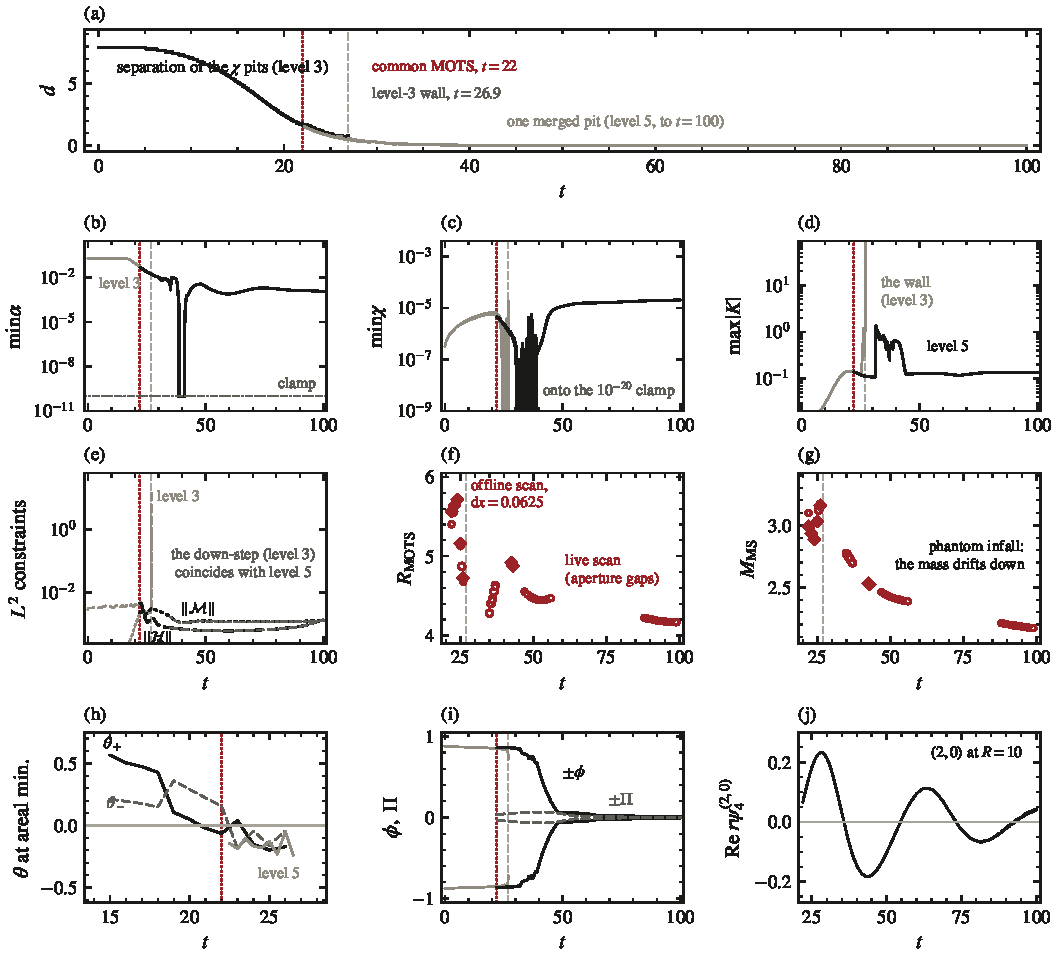
\includegraphics[width=0.80\textwidth]{04_binary_headon/headon_collapse_diagnostics.pdf}
\caption{The head-on merger ($d=8$ from rest, opposite signs): level 5 from $t=0$, no restart, no interior device, clean to $t=100$. Gold rule: common-MOTS formation ($t=22$); dashed rule: the level-3 scout's death ($t=26.91$). (a)~Separation of the $\chi$ pits. (b)--(d)~$\min\alpha$, $\min\chi$ (clamp excursions leave the frame) and $\max|K|$. (e)~Constraint norms: the scout rises to its wall; the level-5 arm and the level-3 down-step arm fall throughout. (f),(g)~Horizon areal radius and Misner--Sharp mass on the scan's MOTS: filled diamonds, offline scans; open circles, live scans; dashed, a linear fit in (f) and the exponential fit of Sec.~\ref{sec:headon:wall} in (g), asymptote dotted. (h)~Null expansions at the areal minimum; no per-mouth scan finds a MOTS. (i)~Scalar extrema. (j)~The $(2,0)$ mode at $R=10$ (conventions of Sec.~\ref{sec:gw}).}
\label{fig:headon_collapse}
\end{figure*}

\subsection{Through the wall to a black hole}
\label{sec:headon:wall}

Five units after the horizon forms, the level-3 scout dies at $t=26.91$ with the classic anatomy---$\chi$ floored at the midpoint, $\max|K|$ running away to $18$, a one-step overflow. The failure is the grid's: at the same time the level-5 arm reads a smooth midpoint (lapse $1.6\times10^{-2}$, $\chi=1.2\times10^{-6}$, $\max|K|=0.11$) and runs to $t=100$ with no restart or interior device and constraint norms falling throughout. The remnant is a trapped ball with no throat left, and its horizon shrinks as it swallows the phantom field: on the level-3 down-step arm, which tracks it to $t=100$, the scan's areal radius falls to $4.17$ by $t=97$, a quarter below its value at formation, still linearly ($-0.0066$ per unit) with no asymptote resolved. $M_{\rm MS}$ falls with it and levels off, fitting $M_\infty+b\,e^{-(t-36)/\tau}$ with $M_\infty=2.160\pm0.006$ and $\tau=19.4\pm0.8$ (a factor $4.8$ better than a line); since $2M_{\rm MS}/R$ falls from $1.23$ to $1.05$ over the fit window as the surface rounds, part of that levelling is the shape systematic of Sec.~\ref{sec:setup:diagnostics}. The spiral remnant ends at the same size ($R=4.15$ at $t=98$--$100$; Sec.~\ref{sec:spiral:inspiral}).

This arm reproduces an earlier level-$3\to5$ restart chain---$(2,0)$ waveforms within $2.9$--$5.4\%$ of peak over the burst, radiated energies within $3$--$8\%$---so the mesh seam carries no result. The exterior is also grid- and device-independent: the level-3 down-step arm agrees on the horizon mass to $1.3\%$ and on the wave to $0.05$--$0.33\%$ of peak over $t=45$--$100$, and fill twins agree with no-fill arms to $0.01\%$ of peak.

\subsection{The half-mass pair}
\label{sec:headon:halfmass}

Halving the throat mass moves everything earlier without avoiding the horizon. At $m=0.5$, $d=6$, the lapse falls from $0.44$ to $0.036$ over $t=7.5$--$13$, the tracker merges the mouths at $t=11.1$, the offline scan finds a common MOTS at $t=12$ ($R=3.83$), and the run dies at $t=14.0$. The death belongs to the pair: the lone $m=0.5$ throat is exact to $0.02\%$ through $t=14$ and fails only at $t=26.3$.

\section{The spiral merger}
\label{sec:spiral}

\subsection{Merger or escape}
\label{sec:spiral:capture}

Varying the tangential momentum at $d=12$ separates plunge from escape. From $p=0.12$ to $0.25$ the pair plunges to a merged core: $p=0.15$ repeats $p=0.12$'s endgame (a plateau at pit separation $0.87$ against $0.81$, then the dive), and at level 5 the pits of $p=0.20$ and $0.25$ coincide by $t\approx41$--$42$, where level 3 stalls them at $1.1$--$1.5$ before its wall. At $p=0.35$ the pair passes at $2.75$ and recedes to $4.0$ by $t=74$ (level 3, stopped there); $p=0.45$ scatters. The merger boundary thus lies between $p=0.25$ and $0.35$, $50$--$70\%$ of the circular value under the combined pull.

The $p=0.45$ fly-by ($L=128$, level 5 to $t=100$) is a scattering pass: closest approach $4.8$ at $t\approx40$, back out to $9.6$ by $t=100$ and still separating. No trapped surface appears on the corrected scans at any time, and the run ends without a NaN. Instead both mouths inflate: from $t\approx43$ the throat lies beyond the scan window ($r\le2.79$), whose edge reading---an upper bound on the throat's areal radius---reaches $33$ by $t=97$, and past $t\approx60$ ``separation'' tracks the $\chi$ pits rather than the throats. On the equatorial slices the pair's scalar dipole is wound into a two-armed trailing spiral, and each mouth drives a crescent of $\chi>1$ ahead of it ($\chi\sim6$ by $t=92$): the encounter ends not as two receding wormholes but as an expanding, orbit-wound cloud of the field that supported them.

\subsection{Plunge and collapse}
\label{sec:spiral:inspiral}

Every ``spiral'' here is a plunge: with $M_{\rm ADM}\simeq1$ per throat, the coordinate separation $d=12$ is $d/M=6$, the innermost-stable-circular-orbit (ISCO) value, and the throat tracks of the momentum scan complete only $0.17$--$0.28$ of a revolution before closest approach ($p=0.20$--$0.35$). Section~\ref{sec:discussion:noinspiral} shows that no wider pair could inspiral instead. The production spiral ($p=0.12$, $L=128$) falls from $d=11.9$ to a single merged pit and collapses at the centre while the throat stays open (Fig.~\ref{fig:spiral_collapse}). The merger's constraint transient at $t=41.2$ is resolved---the level-3 leg reproduces the level-5 norms to a median $3.5\%/0.7\%$---and the collapse after it is clean: the lapse falls to $2.0\times10^{-3}$, $\chi$ reaches its floor at $t=58.4$, and $\max|K|$ grows $24\times$ over $t=50$--$58$ ($0.0084\to6.1$ across the level-5 window) on a wall that lands on the throat; $\phi$ holds $\pm0.89$ while $\Pi$ saturates at $\pm4.1$.

The corrected star-shaped scans find no trapped sphere at $t=55$--$60$ at either resolution, and they are blind here by measurement: every coordinate sphere about the merged pit from $r=1.8$ to $3.4$ carries both signs of $\theta_+$ ($-0.2$ to $+0.15$), so the bracket never closes. The flow finder finds a common MOTS on every surviving death-window slice of the two level-5 arms. On the production chain it has $R=4.83$ at $t=55.0$ ($\theta_-\simeq-0.05$, newly formed; converged from an outer seed at $\ell_{\max}=8$), $4.80$ at $56.0$ and $4.77$ at $57.0$, $5.4$ units before that arm's NaN; on the arm evolved at level 5 from $t=0$ it has $R=4.72\pm0.01$ at $t=59.0$, $0.94$ before its NaN, bracketed by inner and outer seeds, $23\%$ peak-to-peak in coordinate radius about the pit, with $\theta_-=-0.18$. On an exact MOTS $M_{\rm MS}=R/2$: $2.41$ at formation, $2.36$ at $t=59$. On the frozen-core arm's live exterior (fill $r\le1.9$, inside the surface) the remnant at $t=98$--$100$ has $R=4.15$ ($M_{\rm MS}=2.08$), still draining at $0.2\%$ per unit, bracketed by a pointwise-trapped and a pointwise-untrapped surface. The still-open throat ($R=3.87$ at $t=59$ on the second arm) lies inside. At its death the remnant is a black hole containing a wormhole: the head-on's anatomy, reached through a plunge.

\begin{figure}[t]
\centering

\includegraphics[width=0.70\columnwidth]{05_binary_spiral/p012_paper/mouth_growth.pdf}
\caption{Mouth growth in the merging ($p=0.12$) and scattering ($p=0.45$) arms, both from $d=12$ with the same throats; the merger's instrumented re-run carries three refinement levels and the fly-by five, so the shared $\tau$ is a result across two resolutions rather than a one-knob comparison. (a)~Areal radius of one mouth (its twin agrees to $2\times10^{-4}$): solid while the two scan spheres are disjoint, dotted once they overlap; long dash, the common-centre scan. No trapped surface appears on these star-shaped scans, which end at $t=50$ (merger) and $t=100$ (fly-by). (b)~Separation: $p=0.12$ reaches contact, $p=0.45$ misses at $4.8$. (c)~Growth excess $R/R_0-1$ with exponential fits over $t=8$--$25$ (gold): $\tau=3.70$ (merger) and $4.39$ (fly-by).}
\label{fig:mouth_growth}
\end{figure}

The throats grow while the orbit closes. A level-3 re-run carrying per-mouth scans measures each mouth growing $4.2385\to4.7567$ ($+12.2\%$) by $t=28$, the last time the two scan spheres are disjoint, while the separation closes $11.9\to3.6$ (Fig.~\ref{fig:mouth_growth}); the mouths agree to $2\times10^{-4}$, so this is the radial mode. Fitted over $t=8$--$25$, the growth excess $R/R_0-1$ has $\tau=3.70$, against $4.39$ in the fly-by and $5.3$--$5.9$ in isolation: a companion shortens the throat's clock, while the merging and scattering arms agree to $19\%$---the instability belongs to the throat, not to the encounter. The burst of Sec.~\ref{sec:spiral:burst} is thus radiated by throats already a tenth larger than in the initial data.

\begin{figure*}[p]
\centering

\includegraphics[width=0.80\textwidth]{05_binary_spiral/p012_paper/p012_collapse_diagnostics.pdf}
\caption{The production spiral's collapse ($p=0.12$, $d=12$): level 5 from the restart at $t=36$ to the death at $t=60.44$, no interior fill. Rules: the handover at $t=36$ (solid), the merger transient at $t=41.2$ (dashed), the $\chi$ floor at $t=58.4$ (dotted). (a)~Separation of the two $\chi$ pits over the whole history (level 3 carries the plunge; pale past coalescence). (b)--(d)~$\min\alpha$, $\min\chi$ and the scalar extrema. (e)~Constraint norms against $\max|K|$, each $\log_{10}$-scaled onto $[0,1]$. (f)~Radius of the $|K|$ spike (steps, from $t=49.1$, before which the profile is flat) and the $|K|>0.2$ edge (dashed); gold, the throat radius. (g)~Throat areal radius at levels 3 and 5 (circles; the star-shaped scans find no MOTS) and the common MOTS of the shape-free finder (diamonds: filled, this chain; open, the arm evolved at level 5 from $t=0$; Sec.~\ref{sec:spiral:inspiral}). (h)--(j)~Radial anatomy at six equally spaced times, light ($t=36.1$) to dark ($t=60.4$).}
\label{fig:spiral_collapse}
\end{figure*}

\subsection{The curvature wall}
\label{sec:spiral:wall}

No grid carries the spiral through its merger. Restarted from one $t=50$ checkpoint at maximum levels $3$--$7$, every arm of the $p=0.12$ run dies on an $h_{11}$ NaN, and the gains per doubling saturate: $+1.03$, $+2.51$, $+0.53$, $+0.06$ units (Fig.~\ref{fig:spiral_ladder}(a)). Sixteen times the resolution buys $4.13$ units, and halving the time step on level 5 buys $+0.36$, most of the level $5\to6$ gain. The core matter damping moves the wall by less than a unit. Starting refined does not help either: on the doubled box the $p=0.12$ arm evolved at level 5 from $t=0$ dies at $59.94$, against $60.45$ for the production chain restarted at level 5 from $t=36$; a truncation seed two levels smaller buys nothing, so the grid does not seed the wall. The interior freeze then carries the exterior to $t=100$ (Sec.~\ref{sec:spiral:burst}).

The wall is censored. The spiral's common MOTS exists from $t=55.0$ at the latest, $5.4$ units before the production chain's NaN; the head-on's MOTS leads its level-3 death by $4.9$ units; and every collapsed single throat runs clean to $t=100$ behind its horizon. Yet refinement rescues the head-on and never the spiral, although horizon presence, lead time and permanence are matched between them. Censorship is therefore necessary for a finer grid to pass a wall but not sufficient. (The half-mass head-on, with a MOTS at $t=12$ and death at $14.0$, was never re-run at level 5.)

The natural suspect is the slicing. Every arm uses $1{+}\log$ slicing with a Gamma-driver shift, whose slicings can develop coordinate shocks~\cite{alcubierre2003} that refinement resolves rather than cures; a shock at a young, strongly deformed horizon would end every grid. Four gauge choices move the clock without removing the wall (Fig.~\ref{fig:spiral_ladder}(b); the three non-standard arms also carry the core matter damping, which alone moves the level-3 wall by under a unit). At level 3 the spiral dies at $t=43.6$ with the $1{+}\log$ coefficient halved, $49.0$ with the harmonic-class driver $-2\alpha^2K$, $52.1$ in the standard gauge, and $61.9$ with the shift damping raised $\eta=1\to4$, which delays the whole sequence by ${\sim}10$ units (tracker coalescence at $t=41.7$ against $32.1$, $\chi$ floor at $55.6$ against $44.9$). On the head-on control the same knobs give deaths at $25.2$ (harmonic), $26.9$ (standard) and $34.2$ ($\eta=4$), and trapping precedes each: the harmonic arm's MOTS appears at $t=20.8$ with $R=5.47$ against the standard $5.40$---the same surface on an earlier clock, $4.4$ units ahead of the failure---and the $\eta=4$ arm holds whole trapped spheres about the merged pit from $t=30.8$, which bounds a MOTS without locating it (the flow finder stalls there). The head-on's censorship is thus gauge-robust; only its clock moves. For the spiral the flow finder finds no horizon on the harmonic arm's last slice at $\ell_{\max}=6$ or $8$, but no level-3 spiral slice in any gauge has yielded one, so this bounds what level 3 resolves rather than deciding censorship in that gauge. Refinement narrows the gauge spread without closing it: the $\eta=4$ arm restarted at level 5 from $t=50$ dies at $60.04$, $1.9$ units \emph{before} its level-3 clock (a restart at $t=60$ fails at once, at $60.05$), while the standard gauge on the same box and restart dies at $55.60$---a separation of ${\sim}4$ units against $9.8$ at level 3.

The wall is therefore grid-, seed- and device-independent within the Bona--Mass\'o slicings and shift dampings tried: its clock is gauge-dependent, its existence is not. A shock-avoiding or maximal slicing remains untested (Sec.~\ref{sec:discussion:open}).

\begin{figure*}[t]
\centering
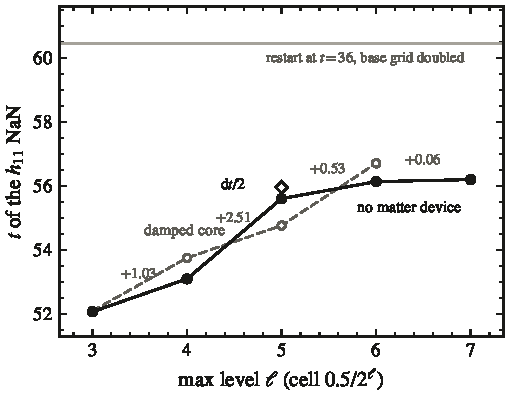
\includegraphics[width=0.80\textwidth]{05_binary_spiral/spiral_refinement_ladder.pdf}
\caption{Death time of the $p=0.12$ spiral under refinement, gauge and start time; every death is an $h_{11}$ NaN except in the $\partial_t\alpha=-\alpha K$ arm, which fails in $K$. (a)~Refinement from one $t=50$ state of the $L=64$ run, maximum level $\ell$ (finest cell $0.5/2^{\ell}$). Filled circles: no matter device, gain per doubling marked; open circles: core matter damping (levels 4--6 share one configuration); open diamond: level 5 at half the time step. These arms left no slices for the shape-free finder. (b)~The same wall under other gauges and start times, one row per gauge. The lapse obeys $\partial_t\alpha=-c\,\alpha^{p}(K-2\Theta)$ and the shift is damped at rate $\eta$; the standard gauge is $c=2$, $p=1$, $\eta=1$, and each other row changes one of the three (and carries the core matter damping, worth under a unit; panel a). Filled circles: level 3 from $t=0$; open circles: level 5 from $t_0$ on $L=64$; open diamonds: level 5 on $L=128$. Level 3: $t=43.6$, $49.0$, $52.1$, $61.9$. Level 5: standard gauge $59.94$ and $60.45$ on $L=128$ ($t_0=0$, $36$) and $55.60$ on $L=64$ ($t_0=50$); $\eta=4$, $60.04$ and $60.05$ ($t_0=50$, $60$).}
\label{fig:spiral_ladder}
\end{figure*}

\section{Gravitational waves}
\label{sec:gw}

Every channel radiates, and the most energetic is the encounter that never forms a horizon. The peak $|r\Psi_4|$ of the dominant mode at the innermost sphere is $4.1\times10^{-2}$ for the fly-by, $2.9\times10^{-2}$ for the spiral, $2.3\times10^{-2}$ for the head-on, $1.1\times10^{-2}$ for the vacuum twin and $2.9\times10^{-3}$ for the collapsing throat (Fig.~\ref{fig:gw_gallery}). Each record propagates outward at $c$ within the output cadence (Fig.~\ref{fig:gw_gallery}, right), but no sphere is asymptotic: the dominant periods are comparable to the extraction radii, and the peak $r\Psi_4$ falls across the spheres by $20\%$ on the head-on and $40\%$ on the fly-by, whose outermost reading drops below the spiral's. We therefore do not extrapolate, and carry the spread over spheres as the near-zone error bar of every energy (Fig.~\ref{fig:gw_ligo}(d)).

In the dominant multipole the fly-by radiates $(4.2$--$7.4)\times10^{-2}\,M$ across its spheres and the spiral up to $2.2\times10^{-2}\,M$, against $2.6\times10^{-3}\,M$ for the vacuum merger control---$16$--$29\times$ and up to $8.5\times$ more. That control matches the spiral; the fly-by's own control is a vacuum binary at $d=12$, $p=0.45$. In vacuum that momentum is unbound (circular $0.204$, parabolic $0.289$), so the black holes start at periapsis and coast apart, radiating $1.05\times10^{-3}\,M$, whereas the drainhole pair falls from $12$ to $4.8$ under a pull six times gravity's. The fly-by thus outradiates a vacuum binary of its own parameters by $40$--$70\times$.

\begin{figure*}[t]
\centering
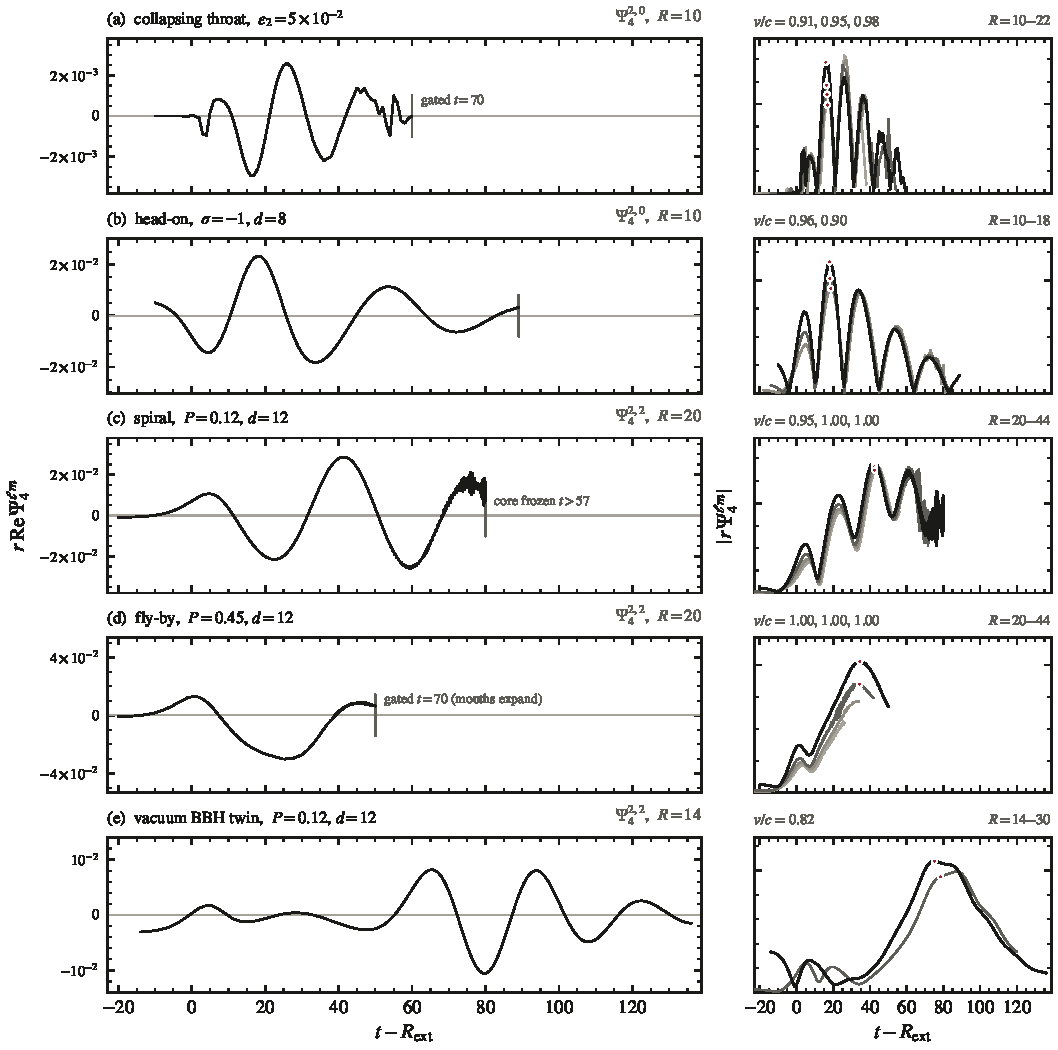
\includegraphics[width=0.80\textwidth]{08_waves/psi4_gallery.pdf}
\caption{The waveform gallery: one row per scenario on one retarded clock. Left: $r\,\mathrm{Re}\,\Psi_4$ of the dominant mode at the innermost sphere, each row on its own scale. Caps mark record ends: the collapsing throat is gated at $t=70$; the spiral record past $t=57$ is carried by the frozen-core arm; the fly-by, complete to $t=100$, is gated at $t=70$ (Sec.~\ref{sec:gw:flyby}). Right: the envelope $|r\Psi_4|$ at every sphere on its own retarded time (ink to faint, inner to outer); a signal moving at $c$ and falling as $1/r$ folds onto one curve. Gold dots: the correlated wavefront. The quoted $v/c$ is the lag of the whole complex waveform between neighbouring spheres, which, unlike peak timing, survives flat-topped envelopes (the vacuum twin's peak times would read $0.57c$, its waveform lag $0.82c$). Speeds: throat $0.91/0.95/0.98$, head-on $0.96/0.90$, spiral $0.95/1.00/1.00$, fly-by $1.00/1.00/1.00$, vacuum twin $0.82$.}
\label{fig:gw_gallery}
\end{figure*}

\begin{figure*}[t]
\centering
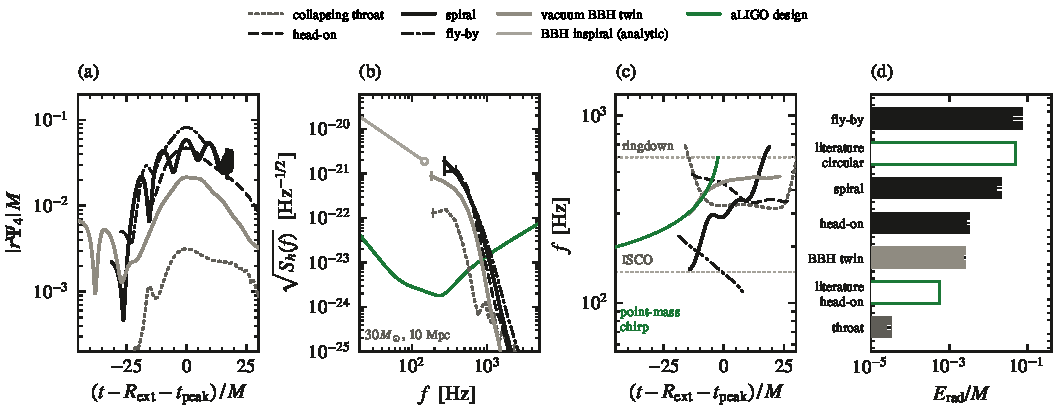
\includegraphics[width=0.80\textwidth]{08_waves/psi4_ligo.pdf}
\caption{Every source at one calibration: total mass $30\,M_\odot$ at $10$ Mpc, each record in units of its own total ADM mass. (a)~Envelopes $|r\Psi_4|M$ at the innermost sphere, aligned at each peak: fly-by loudest ($8.2\times10^{-2}$) to lone throat ($3.1\times10^{-3}$). (b)~Strain amplitude spectral densities over the aLIGO design floor (gold), each from its own low-frequency corner (one cycle per record, ticked). The curves are falling power laws (slopes $-3.3$ to $-5.9$) with no resolved maximum, so any ``peak'' read here is the corner $1/T$. Faint line: the Newtonian inspiral of the same binary, $|\tilde h|\propto f^{-7/6}$ to its ISCO at $147$ Hz. (c)~Instantaneous frequency against the point-mass chirp (gold), the ISCO ($147$ Hz) and the equal-mass Kerr ringdown ($599$ Hz): the vacuum twin climbs the chirp and peaks at $fM=0.065$; no wormhole channel does (Sec.~\ref{sec:ligo:ringdown}). (d)~Energy radiated in the dominant multipole; ticks give the spread over spheres (fly-by $43\%$, the widest). Open gold bars: published equal-mass vacuum values from rest at infinity---head-on infall $5.5\times10^{-4}$, quasi-circular merger $4.84\times10^{-2}$. Energies are band integrals of $|\int r\Psi_4\,\mathrm{d}t'|^2$ over a common retarded window, doubled for $\pm m$; gravitational channel only.}
\label{fig:gw_ligo}
\end{figure*}

\subsection{Collapsing throat}
\label{sec:single:gw}

A lone throat radiates only if its collapse is not spherical. The spherically kicked arm emits nothing above the $\ell=2$ numerical floor, while the same kick with an $\varepsilon_2=0.05$ quadrupole produces a burst of peak $|r\Psi_4|=2.9\times10^{-3}$, $35\times$ the control, carrying $3.2\times10^{-5}\,M$. The burst arrives in radius order at $0.8$--$1.0\,c$, carries the same $r\Psi_4$ to four spheres within $7.2\%$, and is linear in the seed (Fig.~\ref{fig:seed_linearity}): $4.85\times$ for a $5\times$ kick, ratios $1.99/1.97/1.87$ at $R=10/14/18$ for a halved seed, linear to $1$--$16\%$ across $\varepsilon_2=0.005$--$0.05$. The pure quadrupole---$\varepsilon_2=0.01$ with the radial kick removed---radiates the same wave to $2\%$: the deformation, not the kick, is the source. The remnant rings at period $20.6\,M$, $21\%$ shorter than the Schwarzschild fundamental for its horizon mass; the decay time is not measurable on this record.

\begin{figure}[t]
\centering
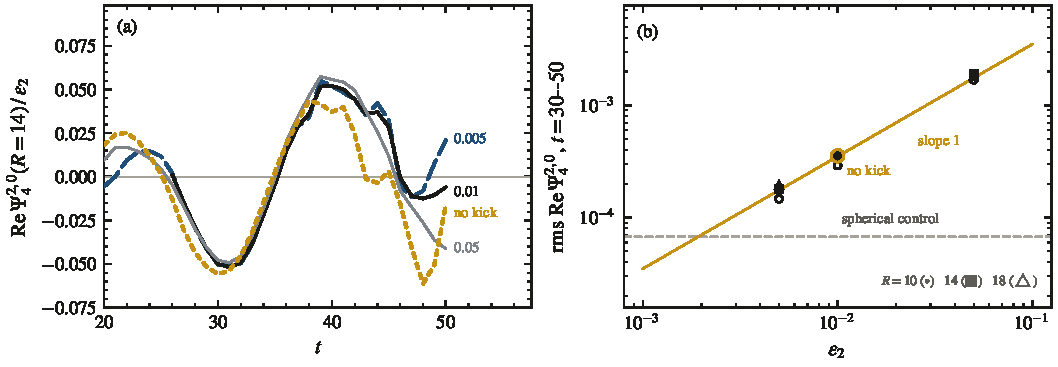
\includegraphics[width=0.70\columnwidth]{01_single_throat/seed_linearity.pdf}
\caption{Linearity of the collapsing throat's wave in its quadrupole seed. (a)~$\mathrm{Re}\,\Psi_4^{2,0}$ at $R=14$, each arm divided by its seed: $\varepsilon_2=0.005$, $0.01$, $0.05$ and the kick-free $0.01$ arm collapse onto one curve. (b)~rms amplitude over $t=30$--$50$ against $\varepsilon_2$ at three spheres, with the slope-one line through the $0.01$ arm. Open circle: the pure quadrupole, within $2\%$ of the kicked arm; dashed rule: the spherical control's floor.}
\label{fig:seed_linearity}
\end{figure}

\subsection{Head-on ringdown}
\label{sec:headon:wave}

The head-on's signal is a bell with no chirp: the $(2,0)$ breathing mode at $R=10$ swings through $+0.023$, $-0.018$, $+0.011$, $-0.006$ at $t=28.2$, $43.6$, $63.5$, $81.7$---a period of ${\sim}31$--$39$, lengthening, the amplitude falling $\times0.6$--$0.8$ per half-swing---and arrives ${\sim}4$ units later per $4$ units of extraction radius ($0.94\,c$), outgoing across all three spheres. On the detector track it is the bell that slows from $486$ to $342$ Hz in Fig.~\ref{fig:gw_ligo}(c).

\subsection{Spiral burst}
\label{sec:spiral:burst}

The spiral's $(2,2)$ burst peaks at $|r\Psi_4|=2.9\times10^{-2}$ and folds onto one curve across $R=20$--$44$ at $v/c=0.95/1.00/1.00$. The record past $t=57$ is carried by the frozen-core arm, whose freeze starts at $t=57$ with its skin at $r=1.9$: its light cone reaches $R=20$ only at $t\approx75$, after the burst peak there ($t\approx62$), and faster gauge modes carry a difference of only $6\times10^{-5}$ of peak ahead of it. A twin with only the fill window moved changes the $(2,2)$ waveform by at most $0.385\%$ of peak (Fig.~\ref{fig:fill_insensitivity}). What the burst is the wave of is half-measured: the remnant is a black hole (Sec.~\ref{sec:spiral:inspiral}), but no surviving slice reaches back to the merger transient at $t=41.2$ that launches the burst, so how much of it left before the horizon closed is unknown.

\begin{figure}[t]
\centering

\includegraphics[width=0.70\columnwidth]{05_binary_spiral/p012_paper/fill_insensitivity.pdf}
\caption{Insensitivity of the spiral's burst to the fill window. (a)~$r\,\mathrm{Re}\,\Psi_4^{2,2}$ at $R=20$ for the freeze arm (fill $1.40/1.90$, ink) and its twin ($1.25/1.75$, gold dots) from the same $t=57$ checkpoint. (b)~Per-sphere envelope of the difference: at most $0.385\%$ of peak at $R=20$ and $0.013\%$ at $R=44$, each front arriving on the fill's causal clock $t=57+(R-1.9)$. The figure certifies the fill's inertness, not a remnant ringdown.}
\label{fig:fill_insensitivity}
\end{figure}

\subsection{Fly-by burst}
\label{sec:gw:flyby}

The $p=0.45$ pass emits a single $(2,2)$ arch of peak $|r\Psi_4|=4.1\times10^{-2}$ with no ringdown---there is no remnant---propagating at $v/c=1.00$ across every sphere pair; in retarded time all four spheres peak together at $t-R\simeq34.5$. The record is complete to $t=100$ with no NaN, but is gated at $t=70$: the mouths' expansion (Sec.~\ref{sec:spiral:capture}) contaminates the innermost sphere, whose $|r\Psi_4|$ stops decaying at $t=76.1$, where the contaminant has grown to equal the decaying burst, $15.5$ units after the $R=20$ peak.

\subsection{Vacuum twin}
\label{sec:controls:bbh}

The vacuum control---same $d$, $p$ and masses, no scalar---behaves as a binary black hole must: it merges, climbs the point-mass chirp $299\to473$ Hz and turns toward the equal-mass Kerr mode, its $\Psi_4$ peak at the textbook $fM=0.065$. The fly-by's peak $|r\Psi_4|$ is $3.8\times$ the twin's and the spiral's $2.7\times$. The twin also calibrates the wavefront method: its flat-topped merger envelope defeats peak timing, so every speed here is a correlated lag (Fig.~\ref{fig:gw_gallery}).

\subsection{Scalar channel and its sign}
\label{sec:gw:scalar}

$\Psi_4$ is blind to a spin-$0$ wave. Two opposite scalar charges---every merging pair here (Sec.~\ref{sec:pair})---carry a dipole, where a vacuum binary's leading moment is the quadrupole. The scalar stream rides the same spheres as $\Psi_4$ on the spiral and fly-by, so the two channels compare sphere by sphere (Fig.~\ref{fig:scalar_channel}). The kinematic flux approximates the scalar energy crossing $S_R$ per coordinate time,
\begin{equation}
F^{\rm geo}_\phi\;=\;-\oint_{S_R}\alpha\,s^i\,T^{(\phi)}_{i\nu}\,t^\nu\,\sqrt{\sigma}\;\mathrm{d}^2x,
\label{eq:scalarflux}
\end{equation}
(canonical sign), with $t^\mu=\alpha n^\mu+\beta^\mu$, $s^i$ the sphere's outward unit normal and $\sqrt{\sigma}$ its area element. Expanded in the evolved variables, $F^{\rm geo}_\phi$ is $F_{\rm kin}$ times a lapse factor (the conformal factors of $s^i$ and $\sqrt\sigma$ cancel at leading order), plus an advective term ${\propto}(\beta^i\partial_i\phi)(s^j\partial_j\phi)$ and the shift's projection $\beta_is^i$ against the gradient energy. At $R=30$ the measured $\alpha$ and $\chi$ lie within $1\%$ of unity, bounding the multiplicative correction at the percent level; the shift terms are not measured.

The channel is dipole-dominated and comparable to the gravitational one. On the fly-by at $R=30$, $\ell=1$ carries the scalar power $\sum_{\ell m}|\dot A_{\ell m}|^2$ to one part in $10^{7}$, the $\ell=1$ signal travels outward at $c$ from $R=14$, and the time-integrated flux to $t=60$ is $|E_\phi|=4.3\times10^{-2}\,M$---$2.3$ times the gravitational energy that has crossed the sphere by then (Fig.~\ref{fig:scalar_channel}(a)). The ratio depends on the cut: it falls to $1.1$ by $t=70$ and $0.8$ by $t=80$ as the rest of the gravitational burst arrives; the wave-zone mode sum gives $1.7$; and the inner sphere returns $3.0$ for the same window. The spiral's scalar record (level 3, to $t=50$) ends before its burst reaches $R=30$ and yields no ratio. We therefore use only the channel's multipole, direction, sign and order of magnitude downstream.

Gravity couples to minus the canonical stress tensor, Eq.~\eqref{eq:phantom}, so the physical energy flux is $-F_{\rm kin}$ and an outgoing scalar wave carries negative energy; what the data establish is that the $\ell=1$ wave is outgoing (on the fly-by, and on the head-on after its horizon forms) and of the size above. If the ADM balance holds with this term, a bound pair emitting it gains energy: the scalar channel pumps the orbit where gravitational radiation damps it, and radiation reaction is \emph{anti-damped}. The same bookkeeping appears at horizons, where swallowing the phantom shrinks the head-on remnant (Sec.~\ref{sec:headon:wall}) and the single-throat horizon regrows as the swallowed field leaves (Sec.~\ref{sec:single:collapse}). That balance, $\dot M_{\rm ADM}=-F_{\rm GW}-F_\phi$, is not closed here---no surface-integral ADM mass was recorded (Sec.~\ref{sec:discussion:open}).

\begin{figure*}[t]
\centering
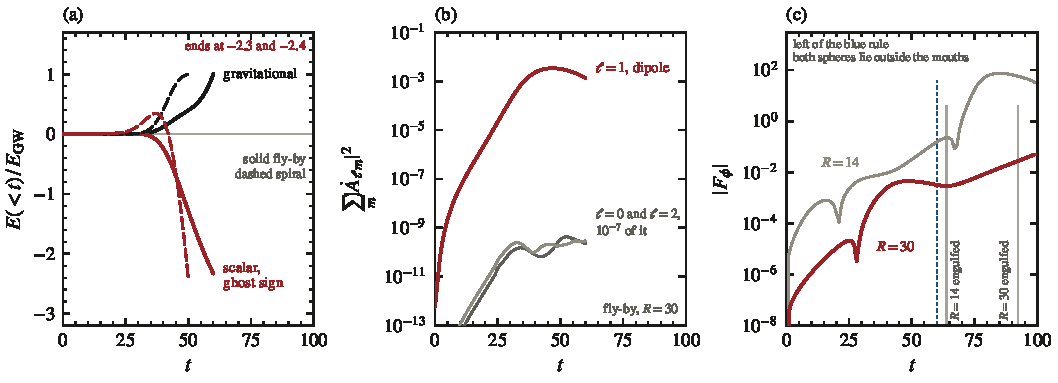
\includegraphics[width=0.80\textwidth]{08_waves/scalar_channel.pdf}
\caption{The scalar channel on the $\Psi_4$ spheres.
(a)~Fly-by energy through $R=30$ in units of the gravitational energy crossed by $t=80$: gravitational (ink) and scalar with its physical sign (gold, Sec.~\ref{sec:gw:scalar}). The ratio $|E_\phi|/E_{\rm GW}$ printed at each cut falls from $3.2$ to $0.8$ as the gravitational burst arrives; past $t\approx80$ the mouths' expansion reaches the sphere. The spiral's scalar record ends before its burst reaches $R=30$ and is not drawn.
(b)~Multipole content, fly-by: $\ell=1$ exceeds $\ell=0$ and $\ell=2$ by $10^{7}$.
(c)~Validity window: $|F_\phi|$ at both spheres, with the times at which the mouths' areal-radius reading (an upper bound) passes each sphere (grey rules); left of the blue rule both spheres lie outside the mouths. The $t=60$ window at $R=14$ gives $3.0$ in place of $2.3$.}
\label{fig:scalar_channel}
\end{figure*}

\subsection{Horizon censorship of the scalar channel}
\label{sec:gw:censorship}

The head-on, re-run at level 5 from $t=0$ with the scalar stream, is the one encounter that forms a horizon early, and the horizon switches the channel off (Fig.~\ref{fig:scalar_censorship}). After the common MOTS closes ($t=21.5$ on this arm's live scan), the mouths' remaining hair leaves as a single $\ell=1$, $m=0$ pulse, cresting later at each sphere in causal order, and the envelope then decays: log-linear fits over $t=30$--$95$ give $\tau=19/23/29$ at $R=10/14/18$, comparable to the $\tau=19.4$ on which the horizon's $M_{\rm MS}$ levels off. The post-horizon energies keep the sign of Sec.~\ref{sec:gw:scalar}, $E_\phi=-0.056/-0.071/-0.075$. Only this window is integrated: before $t=22$ the flux at $R=10$ runs canonically ingoing, the two open mouths' static hair superposing.

Without a horizon the channel does not shut. The fly-by's dipole envelope is still growing at the end of its record. The spiral cannot decide: its horizon exists from $t=55.0$ and its grid dies near $t=60$, five units against a shedding clock of ${\sim}20$; past the wall its curve is the frozen-core arm, which cannot show how a frozen source decays.

The lone throat shows the same contrast. Re-run at level 4 with the scalar stream, the $\varepsilon=+10^{-2}$ throat collapses on schedule---a permanent MOTS from $t=11$, $R$ settling $3.88\to2.45$---and its scalar envelope, after the burst, falls by $30$--$100\times$ across the spheres by $t=80$, with late e-fold times of $5$--$7$. The unkicked level-4 throat, which inflates with no trapped surface by scan or flow finder, instead grows quasi-exponentially in the $\ell=0$ monopole (e-fold ${\approx}5$, shortening across $t=45$--$75$), identically in a box-doubled ($L=128$) copy through $t\approx80$, so the growth is the throat's and not the boundary's or the sponge's; beyond $t\approx80$ the constraint norms grow, and only $t\lesssim80$ is counted. The contrast is confounded with the fate: the horizonless arms are also those whose mouths inflate toward the spheres. What is measured is that the scalar channel shuts off behind a horizon and grows while a throat inflates.

\begin{figure*}[t]
\centering
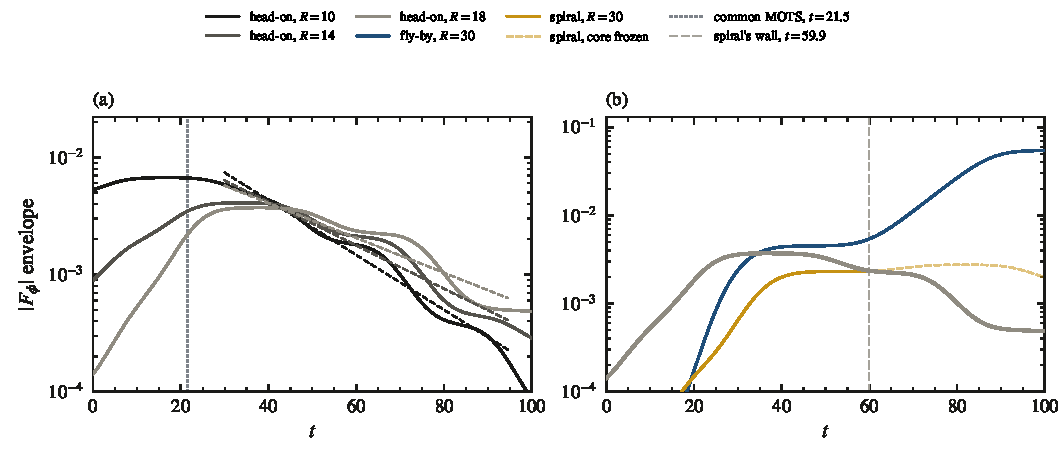
\includegraphics[width=0.80\textwidth]{08_waves/scalar_censorship.pdf}
\caption{Envelope of the scalar flux $|F_\phi|$, horizoned against horizonless arms: a running maximum over $25$ units (one dipole period), smoothed in log amplitude, since the raw flux changes sign every ${\sim}20$ units.
(a)~The head-on (level 5 from $t=0$) at $R=10/14/18$. The common MOTS closes at $t=21.5$ (dotted); the remaining hair leaves as one $\ell=1$ pulse, cresting later at each sphere, then decays (dashed: fits over $t=30$--$95$, $\tau=19/23/29$). The rise before the rule is the open mouths' static hair, canonically ingoing; only the post-horizon window is integrated.
(b)~Each encounter on its outermost sphere (head-on and lone throat $R=18$, fly-by and spiral $R=30$): the fly-by grows to the end of its record; the spiral, with a horizon from $t=55.0$ and too young to shed on a ${\sim}20$ clock, is still climbing at its wall ($t=59.9$, dashed rule), beyond which the frozen-core arm is drawn dashed and carries no claim. Mid-grey: the lone throat twice---the $\varepsilon=+10^{-2}$ level-4 collapse (solid), behind a MOTS from $t=11$, and the unkicked level-4 throat (dotted), which inflates, horizonless, and grows in the monopole (counted to $t\approx80$).}
\label{fig:scalar_censorship}
\end{figure*}

\section{Controls and systematics}
\label{sec:controls}

\subsection{Numerical systematics}
\label{sec:controls:systematics}

Each numerical device has a twin that measures it. The $\chi$ clamp is not load-bearing: twins at $10^{-8}$ and $10^{-20}$ re-converge to four digits after touching the floor. The interior fill is invisible outside: head-on fill and no-fill arms agree to $0.01\%$ of the wave peak, and on the spiral, over the $3.4$ units ($t=57.0$--$60.4$) in which the frozen-core and no-fill arms coexist, the $(2,0)$ and $(2,2)$ modes agree to $0.013\%$ of peak at the innermost sphere, to $10^{-13}$ at the next and bit for bit at the outer two. Two builds differing only in a passive diagnostic produce byte-identical physics streams over $2384$ output rows, certifying both that the diagnostics are non-invasive and that the evolutions are bit-reproducible. The time step is bracketed: multiplier $0.05$ departs from the production $0.02$ at $t\approx33$, and $0.1$ dies at $t=16$. The late $\Psi_4$ floor growth of the single-throat family is sphere-local, not a boundary reflection: the spherical control's $R=14$ sphere climbs four decades while its $R=30$ sphere stays at $1.1\times10^{-3}$; every wave window is gated per sphere ahead of its onset. Matter damping shapes nothing it was meant to.

Two initial-data improvements were tried and rejected. The Helfer superposition correction~\cite{helfer2022} gives better constraints at $t=0$ and worse evolution: it moves the defect from the throats into the fade zone between them, and the orbit stalls instead of plunging (minimum separation $4.6$ at level 3 and $4.9$ at level 4; level 5, stopped at $t=32$, had reached $5.2$); on a fly-by its Hamiltonian norm grows $3.2\times10^{-3}\to1.6\times10^{-2}$ in seven units against a flat plain twin. Constraint-solved data from \texttt{GRTresna} reproduce the drainhole once the outer condition on $\psi_{\rm reg}$ is Robin rather than unity ($\psi$ error $4.9\%\to0.7\%$), but the bridge into the evolution loses the throat at $t=5.3$. Every binary is therefore superposed, its defect declared rather than removed; removing it would buy a fifth of an orbit (Sec.~\ref{sec:discussion:noinspiral}).

\section{Pattern matching against detector data}
\label{sec:ligo}

With the throat mass $M$ as unit, $r\Psi_4$ rescales to strain by $h\propto M/D$ and $f\propto1/M$, so one waveform covers every mass. We confront the rescaled $(2,2)$ and $(2,0)$ waveforms with LIGO--Virgo--KAGRA data products on four fronts: fitting factors against the template family behind the catalogues~\cite{gwtc3}, a matched-filter search of open data~\cite{allen2012}, the ringdown, and unmodelled searches.

Strain comes from fixed-frequency integration~\cite{reisswig2011}, the divisor clamped below each record's lowest resolved frequency (never below one cycle per record). The residual pedestal $|h|(\text{ends})/|h|(\text{peak})$ is $0.02$--$0.07$ for the collapsing throat and the vacuum twin but $0.31$--$0.42$ for the head-on, spiral and fly-by, whose low-frequency strain is therefore an upper bound. The end-to-end test is the vacuum twin: it matches \texttt{IMRPhenomD} at $0.902$--$0.938$ over $60$--$300\,M_\odot$ and recovers its total mass to within $5\%$ up to $200\,M_\odot$ ($+20\%$ at $300\,M_\odot$), so fitting factors are read against that benchmark rather than unity.

\subsection{Fitting factor against the binary-black-hole bank}
\label{sec:ligo:match}

Against a coarse quasi-circular \texttt{IMRPhenomD} bank (total mass $20$--$500\,M_\odot$, mass ratio $1$--$4$, aligned effective spin $-0.5$ to $0.9$) at Advanced LIGO design sensitivity and a common $20$ Hz cutoff (so the pedestal band enters), the channels return fitting factors of $0.49$--$0.82$: collapsing throat $0.54$--$0.79$, head-on $0.49$--$0.75$, spiral $0.54$--$0.80$, fly-by $0.76$--$0.82$. The vacuum twin scores $0.52$--$0.74$ on the same bank, inside that range: the full-bank fitting factor measures record length, not source, and the recovered masses agree ($0.16$--$1.84$ of the true value; the control's $0.11$--$0.53$). No claim that a modelled search would miss these sources follows. Cutting each template to the signal's window removes the duration deficit: the channels then return $0.82$--$0.98$ against the control's $0.93$--$0.95$, so at this duration burst morphology alone does not separate a drainhole channel from a binary black hole. The frequency track does (Sec.~\ref{sec:ligo:ringdown}).

\subsection{A matched-filter search of O3b open data}
\label{sec:ligo:search}

We ran the rescaled waveforms as a search of public Advanced LIGO strain~\cite{gwosc}: five channels times a mass ladder whose neighbouring rungs match at $0.97$ against the live noise curve---$127$ templates---through the standard pipeline~\cite{allen2012,pycbc} (matched filter, Allen's $\chi^2$ test, re-weighted SNR, Hanford--Livingston coincidence, background from $5000$ time slides). All $15$ injections into conditioned O3b strain at optimal SNR $20$ are recovered at $93$--$139\%$ of optimal (median $103\%$) within $3$ ms, with $\chi^2_r=0.6$--$4.8$ (highest on the fly-by); each template is filtered only from its own corner, and the shortest ($5$ ms, four $\chi^2$ bins) is demoted by the veto (SNR $27.8\to14.2$), a sensitivity cost at the lightest fly-by rungs.

In $2.26$ h of coincident CBC\_CAT3 science time there is \emph{no candidate at zero lag}. The background---$13\,920$ accidental coincidences over $471$ days of slid livetime, the loudest at re-weighted SNR $60.4$ (a Hanford glitch at SNR $758$)---caps the smallest reportable false-alarm rate at one per $471$ days. At single-detector SNR $8$ and optimal orientation the median horizon over each mass ladder is $4.8$ Gpc (spiral), $2.5$ (fly-by), $1.8$ (head-on), $1.3$ (vacuum twin) and $0.15$ (collapsing throat); dividing by $2.26$ gives the sky average, and the three pedestal-limited channels are upper bounds. Reach follows where a channel's power lands in the noise curve, not its energy.

\subsection{Ringdown discriminators}
\label{sec:ligo:ringdown}

Where burst shape does not separate the channels, the motion of the frequency does. The vacuum twin peaks at $fM=0.065$ and climbs the point-mass track before turning toward the equal-mass Kerr mode at $fM=0.0885$: a monotone rise, then a fixed ringdown frequency. No drainhole channel does this (Fig.~\ref{fig:gw_ligo}(c)). The head-on's frequency \emph{falls}, $486\to342$ Hz, where a remnant's would sit at its $(2,0,0)$ Kerr value, and mass loss cannot rescue the fit: a shrinking black hole rings \emph{faster}, by $\times1.38$ over this window, while the measurement is $\times0.70$. The fly-by falls further, $227\to115$ Hz, as the pair separates. The collapsing throat rings at a single $335$ Hz ($fM=0.050$), $0.56$ of the equal-mass Kerr mode. A catalogue event whose post-merger frequency holds within a few percent of a Kerr value therefore excludes the head-on channel at that mass. Two limits apply: the spiral's late record is transported by a frozen core from $t=57$ and climbs $151\to679$ Hz without settling, so no spiral ringdown is measured; and the head-on's bell is followed over four swings only, so its decay constant is bounded, not fitted.

\subsection{Burst searches and the stochastic background}
\label{sec:ligo:burst}

Unmodelled searches suit these signals: a burst pipeline asks only for coherent excess power in a time--frequency region, so the missing inspiral costs nothing, and the channels are short and loud in its regime---$5$--$125$ ms across the bank, with the energy within a factor of three in frequency. The detector-independent deliverable is the energy per event in throat-mass units, in the dominant multipole with the sphere spread in parentheses: fly-by $7.4\times10^{-2}\,M$ ($43\%$), spiral $2.2\times10^{-2}\,M$ ($21\%$), head-on $3.3\times10^{-3}\,M$ ($13\%$), collapsing throat $3.2\times10^{-5}\,M$ ($18\%$), vacuum control $2.6\times10^{-3}\,M$ ($5\%$). Since $\Omega_{\rm GW}$ from a population scales as event density times energy per event, these convert any bound on $\Omega_{\rm GW}$---observing-run limits or the nucleosynthesis cap~\cite{lvk2021,pagano2016}---into a bound on the comoving abundance of primordial drainhole encounters, provided the ghost scalar exists at that epoch. They are gravitational energies only; the scalar channel carries comparable energy of the opposite sign (Sec.~\ref{sec:gw:scalar}).

\section{Discussion}
\label{sec:discussion}

All four fates of Sec.~\ref{sec:intro} occur, each with a measured selection rule: the relative scalar sign separates scattering from merger (Sec.~\ref{sec:pair}), the seed's sign separates collapse from inflation (Sec.~\ref{sec:single}), and the orbital momentum separates plunge from escape at $50$--$70\%$ of circular (Sec.~\ref{sec:spiral}). For detection, three results combine: no inspiral exists (Sec.~\ref{sec:discussion:noinspiral}), the wormhole phase is a burst whose frequency falls or drifts where a Kerr remnant's would hold (Sec.~\ref{sec:ligo:ringdown}), and the scalar counterpart decays once a horizon forms (Sec.~\ref{sec:gw:censorship}). A surviving wormhole signature is a drifting-frequency burst with a scalar counterpart; a settled ringdown without one is already the descendant.

\begin{figure*}[!t]
\centering
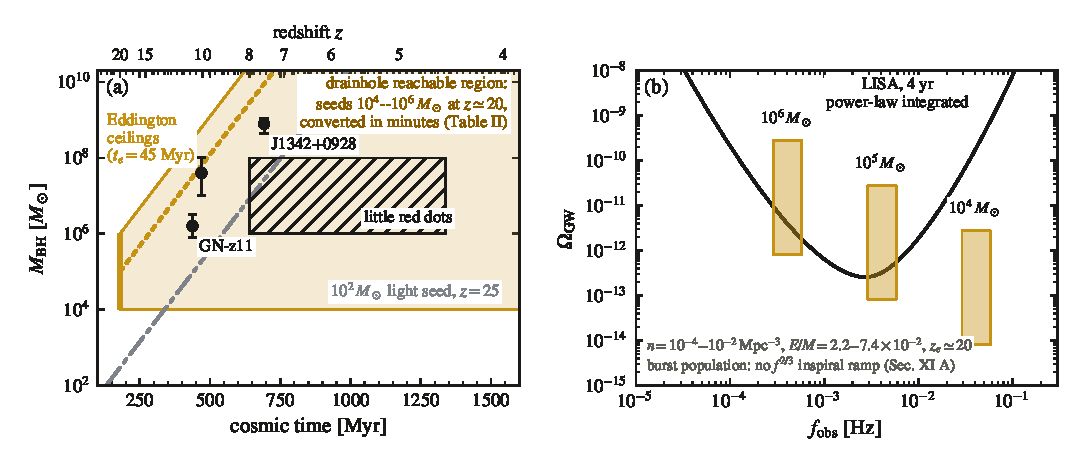
\includegraphics[width=0.92\textwidth]{08_waves/heavy_seeds.pdf}
\caption{The heavy-seed channel from measured numbers. (a)~Seed growth: a drainhole population of $10^{4}$--$10^{6}\,M_\odot$ converts at birth ($z\simeq20$, seconds to minutes; Table~\ref{tab:scales}), so its reachable region (gold) runs from the lightest seed idling to the heaviest seed's Eddington ceiling (Salpeter e-fold $45$ Myr). UHZ1~\cite{bogdan2024,natarajan2024}, GN-z11~\cite{maiolino2024}, the $z=7.5$ quasar J1342$+$0928~\cite{banados2018} and the little-red-dot box~\cite{greene2024,matthee2024} lie inside it; the first three lie \emph{above} the ceiling of a $10^{2}\,M_\odot$ light seed started at $z=25$ (grey), which misses UHZ1 by two decades. (b)~The conversion background $\Omega_{\rm GW}=n\,E_{\rm rad}/[\rho_c(1+z_e)]$ per mass decade: each box spans $E/M=2.2\times10^{-2}$ (spiral) to $7.4\times10^{-2}$ (fly-by) and $n=10^{-4}$--$10^{-2}\,\mathrm{Mpc}^{-3}$, at $f_{\rm obs}=(fM)_{\rm peak}/[M(1+z_e)]$ with $(fM)_{\rm peak}=0.03$--$0.06$. Ink: the four-year power-law-integrated LISA sensitivity from the analytic noise model. The $10^{5}$--$10^{6}\,M_\odot$ boxes straddle it, for conversions at $z_e=20$; conversions at $10^{7}$--$10^{8}\,M_\odot$ fall below the band.}
\label{fig:heavy_seeds}
\end{figure*}

\subsection{No wormhole inspiral}
\label{sec:discussion:noinspiral}

A drainhole binary cannot radiate an inspiral, and the obstruction is a logarithm. In a binary the mouths' unstable mode runs at $\tau=4.39$ (fly-by) and $3.70$ (merger; Sec.~\ref{sec:spiral:inspiral}), faster than the isolated $5.3$--$5.9$; we use $\tau\simeq4.4$. A quasi-circular pair at separation $d$ merges by radiation reaction in $t_{\rm insp}=\tfrac{5}{256}(d/M)^4\,M/\eta$ ($M$ the total mass, $\eta=1/4$): $202$ units from the ISCO, $d/M=6$, and $640$ from $d/M=8$---$1.1$ and $2.25$ orbits at the initial period $T_{\rm orb}=2\pi\sqrt{d^3/M}$, which understates the cycles completed and so is conservative. That gives the instability $t_{\rm insp}/\tau=46$ e-folds at the ISCO and $146$ for a two-orbit inspiral: the mouths reach merger unchanged only if the initial perturbation is below $e^{-46}\simeq10^{-20}$, respectively $10^{-63}$ (with the isolated clock, $10^{-15}$ at the ISCO). Turned around, the lifetime is $\tau\ln(1/\varepsilon)$: seeds of $10^{-6}$, $10^{-10}$ and $10^{-15}$ buy $0.33$, $0.55$ and $0.82$ of one orbit. The orbit's demand grows as $(d/M)^4$ and the throat's endurance as $\ln(1/\varepsilon)$, so no finer grid or quieter data closes the gap: constraint-solved initial data, lowering the seed from the superposition defect to the truncation floor, are worth $\tau\ln(2\times10^{3})\simeq33$ units, a fifth of an orbit.

The inspiral time above is the vacuum quadrupole result, and this binary violates its premises. Its leading radiative moment is a scalar dipole carrying energy comparable to the gravitational channel's (Sec.~\ref{sec:gw:scalar}). Were that energy positive, a reaction two to four times stronger would shorten $t_{\rm insp}$ and relax the ISCO requirement to $11$--$23$ e-folds ($\varepsilon\lesssim10^{-5}$--$10^{-10}$). Its energy is negative, however, so if the ADM balance holds the orbit is pumped rather than drained and no quasi-circular decay exists to compute. A wormhole inspiral fails on the throat's clock and again on the orbit's.

The wormhole-specific signal is therefore a short transient: within a few tens of $M$ each mouth collapses or inflates, and the plunge, burst and conversion of Secs.~\ref{sec:headon}--\ref{sec:gw} are all that this source class emits \emph{as wormholes}. Three qualifications apply. The argument covers a minimally coupled ghost scalar, the matter model of the Gonz\'alez--Guzm\'an--Sarbach analysis; throats held open by rotation, other fields, thin shells or higher-curvature terms are untouched by it. ``No inspiral'' means no \emph{wormhole} inspiral: any long chirp belongs to the objects the throats become. And the seeds here are numerical, which the argument tolerates because its seed dependence is logarithmic and because the superposition defect's excitation of the mode is measured: back-extrapolating the fly-by's mouth growth gives an effective seed of $7\times10^{-4}$, just below the declared-kick decade over which the response is measured linear (Sec.~\ref{sec:single:branching}).

\subsection{Wormhole collapse as a heavy-seed channel}
\label{sec:discussion:seeds}

The collapse branch is a seeding mechanism. A throat converts to a black hole in seconds at $10^{4}$--$10^{5}\,M_\odot$ and in minutes at $10^{6}\,M_\odot$ (Table~\ref{tab:scales}), and the remnant keeps a mass of order its progenitors': the head-on and spiral remnants both end at $R\simeq4.16$ (irreducible mass $2.08$) from pairs of ADM mass $2$, and the lone collapse at $R\approx2.3$--$2.6$ from a throat of mass $1$ (Secs.~\ref{sec:single:collapse}, \ref{sec:headon:wall}, \ref{sec:spiral:inspiral}). The scalar hair leaves on a ${\sim}20\,M$ clock after horizon formation (Sec.~\ref{sec:gw:censorship}), so the remnants then accrete as ordinary black holes. From $10^{4}$--$10^{5}\,M_\odot$ at $z\simeq20$, Eddington-limited growth (Salpeter e-fold ${\simeq}45$ Myr) reaches $10^{9}\,M_\odot$ in $9$--$12$ e-folds, $415$--$520$ Myr, inside the ${\sim}600$ Myr available by $z\simeq7$: no super-Eddington phase is needed, which is what defines a heavy seed~\cite{inayoshi2020} (Fig.~\ref{fig:heavy_seeds}(a)). The channel could thus seed JWST's overmassive black holes and little red dots~\cite{bogdan2024,natarajan2024,greene2024,matthee2024} without an atomic-cooling halo, a critical Lyman--Werner flux, or any baryonic environment.

Halo independence is itself a signature: the seeds predate baryonic structure, so $M_{\rm BH}/M_*$ starts effectively infinite and relaxes downward, making UHZ1's overmassive morphology the generic expectation rather than a tuning. The abundance required is small: one seed per present-day massive galaxy is $n\simeq10^{-4}$--$10^{-2}\,\mathrm{Mpc}^{-3}$ comoving, a dark-matter fraction $f=nM/\rho_{\rm DM}\simeq3\times10^{-11}$--$3\times10^{-7}$ at $10^{4}$--$10^{6}\,M_\odot$. And the channel evades the bound that closes the conventional route: FIRAS $\mu$-distortions exclude primordial black holes of $10^{4}$--$10^{13}\,M_\odot$ formed from Gaussian curvature perturbations at any cosmologically relevant abundance~\cite{nakama2018}, but these black holes form by wormhole collapse, not from enhanced curvature perturbations---the evasion the bubble and domain-wall channels also use~\cite{garriga2016,deng2017}.

The channel radiates, which makes it falsifiable (Fig.~\ref{fig:heavy_seeds}(b)). Each conversion emits the energies of Sec.~\ref{sec:ligo:burst}, so a population contributes $\Omega_{\rm GW}\simeq n\,E_{\rm rad}/[\rho_c(1+z_e)]$ at $f_{\rm obs}=(fM)_{\rm peak}/[M(1+z_e)]$; with the measured $(fM)_{\rm peak}=0.03$--$0.06$ the band is $0.3$--$60$ mHz across $10^{4}$--$10^{6}\,M_\odot$ at $z_e\simeq20$. Taking $E_{\rm rad}/M=2.2\times10^{-2}$ (spiral) to $7.4\times10^{-2}$ (fly-by) at $M=10^{5}\,M_\odot$, $n=10^{-2}\,\mathrm{Mpc}^{-3}$ gives $\Omega_{\rm GW}\sim10^{-11}$ at ${\sim}3$ mHz and $n=10^{-4}$ gives ${\sim}10^{-13}$, against LISA's stochastic sensitivity of $\Omega\sim10^{-13}$--$10^{-12}$ near millihertz~\cite{lisa2017,caprini2018}. Three assumptions carry this. The level and band scale as $1/(1+z_e)$, and $z_e\simeq20$ is about the latest conversion epoch the seed arithmetic allows; a population converting at horizon re-entry would lie far below any band. Lone collapses radiate only $3\times10^{-5}\,M$, which would put the background at $10^{-16}$--$10^{-14}$. And at these abundances the observed rate is only ${\sim}0.05$--$5$ bursts per year, each ${\sim}10^{3}$ s long, so the signal is a sparse burst population rather than a continuous background, and the comparison with a power-law-integrated sensitivity is an optimistic proxy; burst detectability is not computed here. Its spectrum is a pure burst population with no $f^{2/3}$ inspiral ramp (Sec.~\ref{sec:discussion:noinspiral}), unlike any direct-collapse scenario, whose seeds form hydrodynamically. Conversions at $10^{7}$--$10^{8}\,M_\odot$ land at $3$--$60\,\mu$Hz, below the LISA band.

The same events deposit negative energy. The encounters radiate scalar energy comparable to their gravitational energy, with negative sign (Sec.~\ref{sec:gw:scalar}), and an inflating throat sheds its support as a slower monopole of the same sign (Sec.~\ref{sec:single:fate}), so a primordial population fills the early universe with a diffuse negative-energy scalar background. Radiated as massless waves, the prompt deposit redshifts like radiation, to $|\Omega_\phi|\sim\Omega_{\rm GW}\sim10^{-13}$--$10^{-11}$ today---ten orders of magnitude below the dark energy, so the burst channel cannot be $\Lambda$. Whether the deposit back-reacts at $z\simeq20$ is not computed here.

Nothing in the astrophysical mass range survives (Sec.~\ref{sec:single:lifetime}), so every observed supermassive black hole is at most a descendant of this channel, and fits of a static Ellis--Bronnikov metric to the Sgr~A$^*$ or M87$^*$ shadows are excluded within this model. The claim is bounded: the collapse branch is a heavy-seed channel with three measured properties---prompt conversion at comparable mass, halo independence, no $\mu$-distortion---and one testable background; whether it is \emph{the} channel behind the JWST population depends on birth statistics not computed here (Sec.~\ref{sec:discussion:open}).

\subsection{Limitations}
\label{sec:discussion:open}

\emph{Horizon finding.} Most horizon statements rest on star-shaped scans, whose masses carry a shape systematic of up to ${\sim}10\%$ (Sec.~\ref{sec:setup:diagnostics}). The spiral's common MOTS rests on the flow finder alone, on seven slices ($t=55$--$59$ and $98$--$100$) at level-3 sampling of level-5 data, with no slices over $t=59$--$98$ and its birth on records the wall destroyed. The deformable finder overturned the one absence claim it was pointed at; the other records have not been re-searched shape-free. The merging spiral's mouths are measured only to $t=50$, at level 3.

\emph{The wall's mechanism.} Why a censored wall defeats every grid on the spiral but not on the head-on is unexplained (Sec.~\ref{sec:spiral:wall}). The slicing reading is conditional: every arm shares the moving-puncture family, no curvature invariant is recorded at the failure point, and a shock-avoiding or maximal slicing is the untested experiment.

\emph{Energy balance.} $\dot M_{\rm ADM}=-F_{\rm GW}-F_\phi$ is not closed: no surface-integral mass was recorded, and the shift terms of Eq.~\eqref{eq:scalarflux} are unmeasured. $E_\phi$ carries a $30\%$ sphere spread on the binaries; the single throat's is not quoted, because the collapsed arm's post-horizon energy spreads $\times6$ across spheres and the inflating arm is counted only to $t\approx80$.

\emph{Waveforms.} The spiral burst has no resolution test: the level-3 leg ends at $t=50$, before the burst reaches the spheres. No spiral ringdown is measured, and the converted pair's later chirp is not simulated, so these records bound only the wormhole-phase morphology. The low-frequency strain of the head-on, spiral and fly-by is pedestal-limited (Sec.~\ref{sec:ligo}).

\emph{Unattributed numerics.} The late constraint growth on both single-throat branches from $t\approx75$--$80$, and the grid-scale wobble on the outermost head-on sphere after $t\approx80$, are bounded but unexplained.

\emph{Comparisons and astrophysics.} The Gonz\'alez--Guzm\'an--Sarbach comparison is a rate comparison at ${\sim}15\%$; the map between our $(a,m)$ and their perturbation parameters has not been verified term by term. The heavy-seed channel takes the birth abundance $n(M)$ as input, and the collapse fraction of a birth population is not computed: the selection rules are measured, the distribution over them is not, and ambient compression in a radiation-dominated epoch could bias the branch (a throat evolved in a compressive background is the one-arm test). The conversion epoch $z_e$ is assumed, and burst (rather than background) detectability by LISA is not computed. The ghost scalar must exist at that epoch, seed spin is unmeasured, and the cosmological back-reaction of the negative-energy deposit is open.

\section{Reproducibility and cost}
\label{sec:repro}
\label{sec:cost}

Every evolution in Table~\ref{tab:matrix} is one line in a registry shipped with the results pack---its single knob against a named reference, its outcome, its caveats---and every figure is regenerated by a script in the pack from the archived diagnostic streams. The drainhole initial data, the seeds of Sec.~\ref{sec:model:seeds}, the orientation-corrected surface scan and the run parameter files accompany the registry; the code is \texttt{GRTeclyn}~\cite{grteclyn}. The evolutions are bit-reproducible on the production hardware (Sec.~\ref{sec:controls}).

Every evolution ran on one NVIDIA H100 80\,GB device of four-GPU nodes (two 32-core Xeon Platinum 8462Y+ processors), with \texttt{GRTeclyn} built CUDA-native against AMReX~26.02. At $\Delta t=0.02\,\Delta x$ a production arm ($L=64$, $128^3$ base, three refinement levels) advances $12$--$18$ code units per hour, so a $t=100$ evolution costs $6$--$8$ h. Depth is the expense: level-5 arms run at $2$--$4$ units per hour---$28.2$ h for the head-on's $t=0\to100$ and $46.7$ h for the fly-by on the doubled box, which peaks at $58$ of the $80$ GB---and the production spiral's three-stage chain costs $23.5$ h. The $132$ evolutions total $810$ GPU-hours, recomputed from each run's logged speed and time span by a script in the pack; the shakedown adds $9$ h.

\begin{acknowledgments}
This work was supported by Gravity Frontiers
(\url{https://www.gravityfrontiers.org/en}), which funded the underlying
research and the development of the numerical-simulation software. The authors
acknowledge the GRTL Collaboration for \texttt{GRChombo}, \texttt{GRTresna},
and \texttt{GRTeclyn}.
\end{acknowledgments}

% Every float lands inside the body: without this the queue's tail printed
% after the references.
\FloatBarrier

\begin{thebibliography}{99}

\bibitem{wheeler1955}
J.~A.~Wheeler,
\newblock ``Geons,''
\newblock Phys.\ Rev.\ \textbf{97}, 511 (1955).

\bibitem{wheeler1957}
J.~A.~Wheeler,
\newblock ``On the nature of quantum geometrodynamics,''
\newblock Ann.\ Phys.\ (N.Y.) \textbf{2}, 604 (1957).

\bibitem{misner_wheeler1957}
C.~W.~Misner and J.~A.~Wheeler,
\newblock ``Classical physics as geometry,''
\newblock Ann.\ Phys.\ (N.Y.) \textbf{2}, 525 (1957).

\bibitem{roman1993}
T.~A.~Roman,
\newblock ``Inflating Lorentzian wormholes,''
\newblock Phys.\ Rev.\ D \textbf{47}, 1370 (1993).

\bibitem{garriga2016}
J.~Garriga, A.~Vilenkin, and J.~Zhang,
\newblock ``Black holes and the multiverse,''
\newblock J.\ Cosmol.\ Astropart.\ Phys.\ \textbf{02}, 064 (2016).

\bibitem{deng2017}
H.~Deng, J.~Garriga, and A.~Vilenkin,
\newblock ``Primordial black hole and wormhole formation by domain walls,''
\newblock J.\ Cosmol.\ Astropart.\ Phys.\ \textbf{04}, 050 (2017).

\bibitem{kirillov2008}
A.~A.~Kirillov and E.~P.~Savelova,
\newblock ``Dark matter from a gas of wormholes,''
\newblock Phys.\ Lett.\ B \textbf{660}, 93 (2008).

\bibitem{kirillov2011}
A.~A.~Kirillov and E.~P.~Savelova,
\newblock ``Density perturbations in a gas of wormholes,''
\newblock Mon.\ Not.\ R.\ Astron.\ Soc.\ \textbf{412}, 1710 (2011).

\bibitem{ellis1973}
H.~G.~Ellis,
\newblock ``Ether flow through a drainhole: A particle model in general relativity,''
\newblock J.\ Math.\ Phys.\ \textbf{14}, 104 (1973).

\bibitem{bronnikov1973}
K.~A.~Bronnikov,
\newblock ``Scalar-tensor theory and scalar charge,''
\newblock Acta Phys.\ Polon.\ B \textbf{4}, 251 (1973).

\bibitem{morris_thorne1988}
M.~S.~Morris and K.~S.~Thorne,
\newblock ``Wormholes in spacetime and their use for interstellar travel: A tool for teaching general relativity,''
\newblock Am.\ J.\ Phys.\ \textbf{56}, 395 (1988).

\bibitem{visser1995}
M.~Visser,
\newblock \emph{Lorentzian Wormholes: From Einstein to Hawking}
\newblock (AIP Press, Woodbury, NY, 1995).

\bibitem{shinkai2002}
H.~Shinkai and S.~A.~Hayward,
\newblock ``Fate of the first traversible wormhole: Black-hole collapse or inflationary expansion,''
\newblock Phys.\ Rev.\ D \textbf{66}, 044005 (2002).

\bibitem{gonzalez2009}
J.~A.~Gonz\'alez, F.~S.~Guzm\'an, and O.~Sarbach,
\newblock ``Instability of wormholes supported by a ghost scalar field. II. Nonlinear evolution,''
\newblock Class.\ Quantum Grav.\ \textbf{26}, 015011 (2009); see also \textbf{26}, 015010 (2009).

\bibitem{geroch1967}
R.~Geroch,
\newblock ``Topology in general relativity,''
\newblock J.\ Math.\ Phys.\ \textbf{8}, 782 (1967).

\bibitem{tipler1977}
F.~J.~Tipler,
\newblock ``Singularities and causality violation,''
\newblock Ann.\ Phys.\ (N.Y.) \textbf{108}, 1 (1977).

\bibitem{hawking1988}
S.~W.~Hawking,
\newblock ``Wormholes in spacetime,''
\newblock Phys.\ Rev.\ D \textbf{37}, 904 (1988).

\bibitem{zeldovich1967}
Ya.~B.~Zel'dovich and I.~D.~Novikov,
\newblock ``The hypothesis of cores retarded during expansion and the hot cosmological model,''
\newblock Sov.\ Astron.\ \textbf{10}, 602 (1967).

\bibitem{carr_hawking1974}
B.~J.~Carr and S.~W.~Hawking,
\newblock ``Black holes in the early Universe,''
\newblock Mon.\ Not.\ R.\ Astron.\ Soc.\ \textbf{168}, 399 (1974).

\bibitem{carr2021}
B.~Carr, K.~Kohri, Y.~Sendouda, and J.~Yokoyama,
\newblock ``Constraints on primordial black holes,''
\newblock Rep.\ Prog.\ Phys.\ \textbf{84}, 116902 (2021).

\bibitem{caprini2018}
C.~Caprini and D.~G.~Figueroa,
\newblock ``Cosmological backgrounds of gravitational waves,''
\newblock Class.\ Quantum Grav.\ \textbf{35}, 163001 (2018).

\bibitem{nanograv2023}
G.~Agazie \emph{et al.} (NANOGrav Collaboration),
\newblock ``The NANOGrav 15 yr data set: Evidence for a gravitational-wave background,''
\newblock Astrophys.\ J.\ Lett.\ \textbf{951}, L8 (2023).

\bibitem{lisa2017}
P.~Amaro-Seoane \emph{et al.},
\newblock ``Laser Interferometer Space Antenna,''
\newblock arXiv:1702.00786 [astro-ph.IM] (2017).

\bibitem{lvk2021}
R.~Abbott \emph{et al.} (LIGO Scientific, Virgo and KAGRA Collaborations),
\newblock ``Upper limits on the isotropic gravitational-wave background from Advanced LIGO and Advanced Virgo's third observing run,''
\newblock Phys.\ Rev.\ D \textbf{104}, 022004 (2021).

\bibitem{pagano2016}
L.~Pagano, L.~Salvati, and A.~Melchiorri,
\newblock ``New constraints on primordial gravitational waves from Planck 2015,''
\newblock Phys.\ Lett.\ B \textbf{760}, 823 (2016).

\bibitem{allen2012}
B.~Allen, W.~G.~Anderson, P.~R.~Brady, D.~A.~Brown, and J.~D.~E.~Creighton,
\newblock ``FINDCHIRP: An algorithm for detection of gravitational waves from inspiraling compact binaries,''
\newblock Phys.\ Rev.\ D \textbf{85}, 122006 (2012).

\bibitem{reisswig2011}
C.~Reisswig and D.~Pollney,
\newblock ``Notes on the integration of numerical relativity waveforms,''
\newblock Class.\ Quantum Grav.\ \textbf{28}, 195015 (2011).

\bibitem{pycbc}
S.~A.~Usman \emph{et al.},
\newblock ``The PyCBC search for gravitational waves from compact binary coalescence,''
\newblock Class.\ Quantum Grav.\ \textbf{33}, 215004 (2016).

\bibitem{gwosc}
R.~Abbott \emph{et al.} (LIGO Scientific, Virgo and KAGRA Collaborations),
\newblock ``Open data from the third observing run of LIGO, Virgo, KAGRA and GEO,''
\newblock Astrophys.\ J.\ Suppl.\ \textbf{267}, 29 (2023).

\bibitem{gwtc3}
R.~Abbott \emph{et al.} (LIGO Scientific, Virgo and KAGRA Collaborations),
\newblock ``GWTC-3: Compact binary coalescences observed by LIGO and Virgo during the second part of the third observing run,''
\newblock Phys.\ Rev.\ X \textbf{13}, 041039 (2023).

\bibitem{misner_sharp1964}
C.~W.~Misner and D.~H.~Sharp,
\newblock ``Relativistic equations for adiabatic, spherically symmetric gravitational collapse,''
\newblock Phys.\ Rev.\ \textbf{136}, B571 (1964).

\bibitem{hochberg_visser1998}
D.~Hochberg and M.~Visser,
\newblock ``Dynamic wormholes, antitrapped surfaces, and energy conditions,''
\newblock Phys.\ Rev.\ D \textbf{58}, 044021 (1998).

\bibitem{hawking1971}
S.~W.~Hawking,
\newblock ``Gravitational radiation from colliding black holes,''
\newblock Phys.\ Rev.\ Lett.\ \textbf{26}, 1344 (1971).

\bibitem{bowen_york1980}
J.~M.~Bowen and J.~W.~York,
\newblock ``Time-asymmetric initial data for black holes and black-hole collisions,''
\newblock Phys.\ Rev.\ D \textbf{21}, 2047 (1980).

\bibitem{helfer2022}
T.~Helfer, U.~Sperhake, R.~Croft, M.~Radia, B.-X.~Ge, and E.~A.~Lim,
\newblock ``Malaise and remedy of binary boson-star initial data,''
\newblock Class.\ Quantum Grav.\ \textbf{39}, 074001 (2022).

\bibitem{alic2012}
D.~Alic, C.~Bona-Casas, C.~Bona, L.~Rezzolla, and C.~Palenzuela,
\newblock ``Conformal and covariant formulation of the Z4 system with constraint-violating solutions,''
\newblock Phys.\ Rev.\ D \textbf{85}, 064040 (2012).

\bibitem{bona1995}
C.~Bona, J.~Mass\'o, E.~Seidel, and J.~Stela,
\newblock ``New formalism for numerical relativity,''
\newblock Phys.\ Rev.\ Lett.\ \textbf{75}, 600 (1995).

\bibitem{campanelli2006}
M.~Campanelli, C.~O.~Lousto, P.~Marronetti, and Y.~Zlochower,
\newblock ``Accurate evolutions of orbiting black-hole binaries without excision,''
\newblock Phys.\ Rev.\ Lett.\ \textbf{96}, 111101 (2006).

\bibitem{baker2006}
J.~G.~Baker, J.~Centrella, D.-I.~Choi, M.~Koppitz, and J.~van~Meter,
\newblock ``Gravitational-wave extraction from an inspiraling configuration of merging black holes,''
\newblock Phys.\ Rev.\ Lett.\ \textbf{96}, 111102 (2006).

\bibitem{grteclyn}
GRTL Collaboration,
\newblock \texttt{GRTeclyn},
\newblock \url{https://github.com/GRTLCollaboration/GRTeclyn}.

\bibitem{amrex}
W.~Zhang \emph{et al.},
\newblock ``AMReX: a framework for block-structured adaptive mesh refinement,''
\newblock J.\ Open Source Softw.\ \textbf{4}, 1370 (2019).

\bibitem{grchombo}
T.~Andrade \emph{et al.},
\newblock ``GRChombo: an adaptable numerical relativity code for fundamental physics,''
\newblock J.\ Open Source Softw.\ \textbf{6}, 3703 (2021).

\bibitem{shirokov2026}
N.~M.~Shirokov,
\newblock ``Wormhole dynamics: nonlinear collapse and gravitational-wave emission,''
\newblock arXiv:2604.00071 [gr-qc] (2026).

\bibitem{shirokov2026b}
N.~M.~Shirokov,
\newblock ``The Bondi dipole in full numerical relativity: a self-accelerating positive--negative mass binary,''
\newblock submitted (2026).

\bibitem{bogdan2024}
\'A.~Bogd\'an \emph{et al.},
\newblock ``Evidence for heavy-seed origin of early supermassive black holes from a $z\approx10$ X-ray quasar,''
\newblock Nat.\ Astron.\ \textbf{8}, 126 (2024).

\bibitem{natarajan2024}
P.~Natarajan, F.~Pacucci, A.~Ricarte, \'A.~Bogd\'an, A.~D.~Goulding, and N.~Cappelluti,
\newblock ``First detection of an overmassive black hole galaxy: UHZ1---evidence for heavy black hole seeds from direct collapse?,''
\newblock Astrophys.\ J.\ Lett.\ \textbf{960}, L1 (2024).

\bibitem{greene2024}
J.~E.~Greene \emph{et al.},
\newblock ``UNCOVER spectroscopy confirms the surprising ubiquity of active galactic nuclei in red sources at $z>5$,''
\newblock Astrophys.\ J.\ \textbf{964}, 39 (2024).

\bibitem{matthee2024}
J.~Matthee \emph{et al.},
\newblock ``Little red dots: an abundant population of faint active galactic nuclei at $z\sim5$ revealed by the EIGER and FRESCO JWST surveys,''
\newblock Astrophys.\ J.\ \textbf{963}, 129 (2024).

\bibitem{maiolino2024}
R.~Maiolino \emph{et al.},
\newblock ``A small and vigorous black hole in the early Universe,''
\newblock Nature \textbf{627}, 59 (2024).

\bibitem{banados2018}
E.~Ba\~nados \emph{et al.},
\newblock ``An 800-million-solar-mass black hole in a significantly neutral Universe at a redshift of 7.5,''
\newblock Nature \textbf{553}, 473 (2018).

\bibitem{inayoshi2020}
K.~Inayoshi, E.~Visbal, and Z.~Haiman,
\newblock ``The assembly of the first massive black holes,''
\newblock Annu.\ Rev.\ Astron.\ Astrophys.\ \textbf{58}, 27 (2020).

\bibitem{nakama2018}
T.~Nakama, B.~Carr, and J.~Silk,
\newblock ``Limits on primordial black holes from $\mu$ distortions in cosmic microwave background,''
\newblock Phys.\ Rev.\ D \textbf{97}, 043525 (2018).

\bibitem{alcubierre2003}
M.~Alcubierre,
\newblock ``Hyperbolic slicings of spacetime: singularity avoidance and gauge shocks,''
\newblock Class.\ Quantum Grav.\ \textbf{20}, 607 (2003).

\end{thebibliography}

\end{document}
